% !TEX root = thesis.tex
\startchapter{Do Developers Talk about Change-Sets?}
\label{chap:talk}
Knowing that our approach can generate statistically significant recommendations is only one necessary step towards showing its usefulness.
As Murphy and Murphy-Hill~\cite{murphy:rsse:2010} pointed out recommendation become of little use once developer reject them.
Thus in this chapter we peruse the following research question:

\begin{description}
  \item[RQ 2.2:] Do developer accept recommendations based on software changes to increase build success? 
\end{description}

We want developer to communicate as soon as we suspect that the likelihood for a build to succeed diminishes.
But currently our investigation only took a very technical stance and ignores many other criteria that might be of relevance to developers.
For instance, it is unlikely that every build is of equal importance.
Furthermore, we also think that developers opinion of each other play a role, such as trust and respect.
Therefore, it is important to explore those less technical aspects of developer relationship to gain a better understanding on when to deliver a recommendation.

% give chapter overview
In the remainder of this chapter, we start with detailing some related work into team coordination (Section~\ref{ch9:bg}).
Subsequently, we briefly go over the study design that is relevant to exploring our research question (Section~\ref{sec:studydesign}).
Then, we go over the findings we obtained in Section~\ref{sec:findings} followed by some general recommender system design guidelines derived from the results and threats to validity in Section~\ref{sec:sub:tools} and Section~\ref{sec:threats} respectively.
We conclude this chapter with offering an answer to our research question and leading into the subsequent Chapter~\ref{chap:actionable} (Section~\ref{sec:conclusions}).

\section{Background}
\label{ch9:bg}
%old introduction
For all but the most trivial programs, software development today is a collaborative activity. The members of software teams must coordinate and communicate, often intensely, if their projects are to reach a satisfactory conclusion.
Previous research has shown that communication among developers has a profound influence on several aspects of software development~\cite{hinds:cscw:2006,wolf:icse:2009}.

Despite this acknowledged importance of communication in software teams, our understanding of communication behaviour is still very limited. Ko \emph{et al.}~\cite{ko:icse:2007} point out that developers often require information about the work output of their peers.  We know little about why developers act upon this requirement. What causes developers to seek information in some cases, but not in others? There are a multitude of potential factors: the closeness of their peers' work with their own, the expertise of the developers, their physical proximity, their level of workload, and even, perhaps, the time of day. By identifying which factors actually influence the likelihood that a developer will request information about the events surrounding her, we might better understand the nature of software-centric information-seeking behaviour. This increased understanding allows us to develop improved recommender systems that enable developers to coordinate their activities efficiently.

% related work start
Overall, this research builds upon the growing body of work that studies coordination and communication in software organizations, which have long been recognized as playing central roles in leading software projects to success, e.g.~\cite{kraut:1995coordination,curtis:acm:1988}.  

Earlier we reported on investigations of the RTC project repositories revealed a significant relationship between gaps in communication structures and build success (Chapter~\ref{chap:stc-net2} and~\ref{chap:stc-net}). Therefore we proposed a recommendation system that allows team members to learn about who they should talk with in order to avoid build failures~\cite{schroeter:rsse:2008}. This recommendation system should focus on changesets and analyze significant differences between code dependencies and team communication structure to identify anti-patterns that the developers should attempt to break.
The basis for this principle is derived from Conway's Law~\cite{conway:datamination:1968} and by the model of socio-technical congruence proposed by Cataldo et al~\cite{cataldo:cscw:2006,cataldo:esem:2008}.
The model compares the communication network to the code dependency network and derives insights with respect to productivity from the gaps between those networks.

In order to build a good recommendation system, however, one needs to go beyond providing valuable information. As Murphy and Murphy-Hill show~\cite{murphy:rsse:2010}, we need developers to trust the recommender system: delivering the right recommendation at the right time is one important way to build such trust. Unfortunately, recommender systems often fall short on this front, saturating the developer with recommendations they neither need nor want, or presenting recommendations at inappropriate times. It is therefore important to know when developers actually need information, and what factors influence them to seek information. There are many potential factors that could change the likelihood that developers would want to obtain further information, and we do not have a sense, other than our intuition, to learn which factors are actually important and which are not.

Related work has examined factors that influence communication among software developers. For instance, while APIs are intended to reduce coordination complexity among development teams, they also introduce barriers that hinder communication between teams by obscuring dependencies~\cite{souza:cscw:2004,desouza:fse:2004}.
Software architecture, organizational structure and project age are also factors that influence communication and the awareness that developers have of each other's work~\cite{cleidson:tse:2011}. 
Processes, in particular, are often used to influence the communication among team members to reduce information overload~\cite{fussell:cscw:1998}, and geographic distance has been shown to affect communication, but its effects vary between projects~\cite{herbsleb:icse:2001,wolf:spip:2008}.
Nakakoji et al~\cite{nakakoji2010:rdc} distilled the current knowledge about communication among developers into a set of guidelines to design tools and processes that facilitate effective expertise communication.
Those studies, and to our knowledge, literature in software engineering in general, only address communication on a project-wide level. However, to fully understand, and thus offer actionable knowledge to developers, we need to know what influences an individual developer's information-seeking behaviour.
We surveyed literature to compile a list of possible information-seeking triggers spanning change-related (such as code metrics), developer-related (such as experience level) and process-related (such as peer reviews) factors.



\section{Study Design}
\label{sec:studydesign}
We complement our previous analysis of the RTC electronic repositories with rich qualitative data from interviews and observations, considering that much information on a project's lifecycle is not recorded in its repositories~\cite{aranda:icse:2009}. We focused on studying what factors cause a developer to seek information about a changeset, since changesets are the smallest units of change to a project that directly impact other developers.

Our research question calls for a mixed methods empirical study. Therefore, we collect data about the team's information-seeking behaviour from three different sources.
First, the author of this thesis was embedded in a sub-team of the RTC team as a participant-observer for four months.
Second, we deployed a survey with the entire development team to validate some of the findings from the observations.
Third, we conducted interviews with the developers from one component team to obtain richer information about their communication behaviour.


\subsection{Data Collection}
We used a mixed methods approach to answer our research question. We obtained data from three sources: participant observation, a survey, and a set of interviews with RTC team members.

\subsubsection{Participant-Observation}
The  author of this thesis joined one of the RTC development sites in Europe for a four-month period in the Fall of 2010. He was involved as an intern with this development team helping with minor bug fixes, feature development, and testing, and thus was in a position to directly participate in the project development and communication activities. Our data collection opportunities were thus much richer than in typical observations conducted over shorter periods of time, or that do not involve active participation in the project.  During his period as a participant-observer, Adrian kept a daily activity log, recording any information of relevance to the communication behaviour of his team.

The observation period coincided with the months prior to a major release and during which the team focused on extensive testing rather than new feature development. As such, the majority of our observations are concerned with activities around testing the integration of RTC with other IBM Rational products, and it offered the experience of collaborating with many developers from different teams and across the remote sites. Finally, in the one month following the release, Adrian also participated in the development of a feature for the upcoming version of the product.

The team in which he was embedded had the responsibility to develop the task management and the planning components of RTC. There were ten developers at the site, including two novices that had recently joined the team and eight experienced developers. The team includes RTC's three senior project management members, who play a major role in planning the entire product's architecture and development.


\begin{sidewaystable}
\centering
%\subfloat[Process-related items and quotes]{
\small
\centering
\begin{tabular}{l@{\hspace{7pt}}l@{\hspace{-20pt}}r}
\toprule
Survey Items & Interview Quotes (I)/Participant Observation Quotes (O) & Mean Rank\\
\midrule
Release endgame & (O) \emph{``Adrian, in the endgame we only do minimal changes. Is your change minimal?''}& 3.79\\%319\\
To review the change &(I) \emph{``I often lack sufficient understanding of the part of the code I'm reviewing.''}& 5.00\\%311\\
To approve the change &--- & 5.11\\%298\\
Late milestone &--- & 5.14\\%293\\
During iteration endgame &(O) \emph{``Adrian, in the endgame we only do minimal changes. Is your change minimal?''}& 5.42\\%288\\
Obtain a review for the change &(O) \emph{``It is demotivating to get a reject, thus I talk to my reviewer beforehand.''}& 5.55\\%287\\
Obtain an approval for the change &(O) \emph{``I already fixed it, but I  need to convince my team lead to give me approval.''}& 5.72\\%281\\
Related work item has high severity &--- & 6.00\\%246\\
Verify a fix &(I) \emph{``Often I need to ask how I can tell that a change-set actually fixed the bug.''}& 6.37\\%235\\
Topic of work item the change is attached to &--- & 7.64\\%181\\
Priority set by your team lead&--- & 8.55\\%152\\
Role of the committer (e.g. developer) &--- & 9.00\\%145\\
Early in an iteration &(I) \emph{``... there are weeks I sometimes don't talk to my colleagues at all.'''}& 11.24\\%66\\
Early milestone &--- & 12.10\\%60\\%\emph{``''}
\bottomrule
\end{tabular}
\label{tab:sub-process}
%}\vspace{0pt}
\caption{Process-related items and quotes}
%\end{table}
\end{sidewaystable}

%\begin{table}[t]
\begin{sidewaystable}
%\subfloat[Developer-related items and quotes]{
\small
\centering
\begin{tabular}{l@{\hspace{5pt}}l@{\hspace{-10pt}}r}
\toprule
Survey Items & Interview Quotes (I)/Participant Observation Quotes (O) & Mean Rank\\
\midrule
Author is inexperienced &(O) \emph{``Adrian, please put me always as a reviewer on you change-sets.''}& 2.60\\%385\\
Author recently delivered sub-standard work&(I) \emph{``She just changed teams and still needs to get used to this component.''}& 3.04\\%335\\
Author is not up to date with recent events &(I) \emph{``After you return from vacation we ensure you follow new decisions.''}& 3.15\\%329\\ 
You do not know the change-set author &(I) \emph{``I'd be very irritated if someone other than [...] would touch my code.''}& 5.09\\%269\\	
Author is currently working with you &(O) \emph{``We sometimes discuss changes we made to brag about a cool hack.''}& 5.56\\%226\\	
Author part of same feature team &--- & 6.00\\%190\\ 	
Author part of your team &--- & 7.00\\%188\\ 		
Worked with author before &--- & 7.77\\%165\\ 			
Busyness of yourself &(I) \emph{``If I see a problematic change-set, I'll ask for clarifications even if I'm busy.''}& 8.05\\%164\\
Busyness of the author &(I) {\small\emph{``If I need to know why an author made that change I just contact him.''}}& 8.55\\%147\\
Met in person &(I) \emph{``I've worked with him for 5 years now but never even met him.''}& 9.57\\%117\\
Physical location &(O) \emph{``Here, America or Asia, I don't care, I ping them when they are online.''}& 10.14\\%112\\ 
Author is experienced &--- & 11.00\\%93\\ %\emph{``''}		
Author recently delivered high-quality work &--- & 11.09\\%86\\%\emph{``''}
\bottomrule
\end{tabular}
\label{tab:sub-social}
%}\vspace{0pt}
\caption{Developer-related items and quotes}
%\end{table}
\end{sidewaystable}

%\begin{table}[t]
\begin{sidewaystable}
%\subfloat[Code-change-related items and quotes]{
\small
\centering
\begin{tabular}{l@{\hspace{-10pt}}l@{\hspace{-20pt}}r}
\toprule
Survey Items & Interview Quotes (I)/Participant Observation Quotes (O) & Mean Rank\\
\midrule
Changed API &(O) \emph{``Adrian, why did you change that API?''} [The RTC team avoids changing API.] & 2.84\\%390\\            	
Don't know why code was changed &(O) \emph{``I don't see a reason why you changed that code, you sure you needed to?''}& 3.00\\%348\\ 
Affects frequently used features &(I) \emph{``Before I ok a fix [even to a main feature], I ask if there is a workaround.''} & 4.10\\%325\\ 
Complex code &--- & 4.89\\%289\\	%\emph{``''}
Introduced new functionality &--- & 6.14\\%260\\ %\emph{``''}
Is used by many other methods &(O) {\small\emph{``Why did you fix this part? The bug is not in this part of the code,}}& 6.41\\%240\\ 
&\emph{ it is used and tested a lot.''}&\\
Your code was changed &(I) \emph{``I'd be very irritated if someone other than [...] would touch my code.''}& 6.42\\%232\\ 
Stable code was changed &(O) {\small\emph{``Why did you fix this part? The bug is not in this part of the code, }}& 6.62\\%213\\
&\emph{it is used and tested a lot.''}&\\
Change unlocks previously unused code &--- & 7.42\\%192\\ 
A bug fix &--- & 8.61\\%162\\%\emph{``''}	
A re-factoring &(O) \emph{``I separate a re-factoring from a fix so that people can }& 9.15\\%152\\
&\emph{ask me questions about the fix.''}&\\
Frequently modified code was changed &(I) \emph{``I like to know where the `construction sites' of the project are.''}& 10.35\\%118\\ 
Code is used by few other methods &--- & 10.96\\%94\\ 	
Simple code was changed\phantom{abcdefgheabcdefghe} &--- & 12.57\\%58\\   %23 characters	43
%Author recently delivered high-quality work	
\bottomrule
\end{tabular}
\label{tab:sub-technical}
\caption{Code-change-related items and quotes}
%}\vspace{-10pt}
\label{tab:surveyfactors}
%\end{table}
\end{sidewaystable}

\subsubsection{Interviews}
We conducted interviews with ten developers of the RTC team to inform our observational findings. The setting for the interviews was slightly unusual, and beneficial from a research perspective, since the first author's participant-observation allowed him to develop working relationships during his stay at the team, and to delve into a discussion of complex communication issues without needing to spend time understanding the basic context of the team.

In the interviews, we requested developers to provide details into their communication dynamics through a narration of ``war stories'' that directly related to communication among developers. ``\emph{War stories}'' are events that left an impression on the respondent. War stories emphasize specific events that they witnessed or took part in~\cite{lutters:ist:2007}; their narrative is particularly powerful at uncovering the elements of the stories that are relevant to the respondents. The interviews lasted between thirty minutes and one hour, and they were conducted at the end of the observation period. 


\subsubsection{Survey}
To complement the insights we obtained from the observations and interviews, we deployed a survey with the entire RTC team at the end of our observation period. The survey was designed iteratively and piloted with a European team, and intended to collect input about which factors increase the likelihood of a developer requesting information about a changeset from the changeset author. The items we included in the survey were in the categories of code-related, developer-related and process-related items. Each category included 14 items, as shown in Table~\ref{tab:surveyfactors}. \emph{Code-change related} items describe the changeset delivered or the code that the changeset modifies or affects. \emph{Developer-related} items relate to
the developers that delivered a changeset, the developer requesting the
information, and their relation to each other. Finally, \emph{process-related} items relate to the development phase in effect when the changeset was delivered, and to items relating to process requirements or practices. For each of the three categories, the survey asked the developers to rank each item in the category according to how strongly it increases their likelihood of requesting information about a changeset. 

We initially formulated our list of items from an analysis of the current literature on coordination and communication, as well as from our own previous research. We then refined the list of items through piloting and discussions with the development team. An initial version of the survey included fifty-nine items; the refined list had forty-two. Besides reducing the number of items in our list, the pilot survey led us to add several process-related items, as well as to change the format of the question (the initial survey had a battery of questions with Likert-scale answers; the final survey asked respondents to rank each item in comparison to the rest in its own category).

We deployed the survey through a web form, and invited the entire distributed RTC development team to participate. We sent a reminder one month later to increase the response rate. We obtained 36 responses to the survey; approximately a 25\% response rate.
Of the 36 respondents, 26 are located in North America, 5 are located in Europe, and 5 are located in Asia. Furthermore, 22 of the respondents are developers, 5 team leads, 5 component leads and project management committee, and 4 respondents withheld their information.

\subsection{Analysis} 
For our data analysis, we transcribed the interviews, and then coded both the interviews and the participant-observation notes. From the codes we created categories, which we cross-referenced to the survey rankings. We used an open coding approach, during which we assigned codes to summarize incidents in sentences and paragraphs of the transcribed interviews that relate to our research question.

We calculated the ranking of the survey items for each category by calculating the mean over all ranks given by developers to a survey item (see Table~\ref{tab:surveyfactors}).
Table~\ref{tab:sparkle} shows the distribution of the rankings for each survey item.

During our analysis, we derived a set of factors affecting communication behaviour based on our list of survey items and qualitative data from our interviews and observations. Whenever possible, we triangulated our findings using all our data sources. We tried to ensure that all of our findings were supported by at least two data sources; none of the findings we report were challenged by any of our data sources. 


\section{Findings}
\label{sec:findings}
The evidence collected from our survey, interviews, and participant observation allowed us to derive seven factors that affect communication behaviour in software organizations, which we outline below. In the remainder of this section, text in italics refers to survey items that can be found in Table \ref{tab:surveyfactors}. Text in italics and around quotation marks denotes interview fragments.

\begin{figure}[tb]
\centering
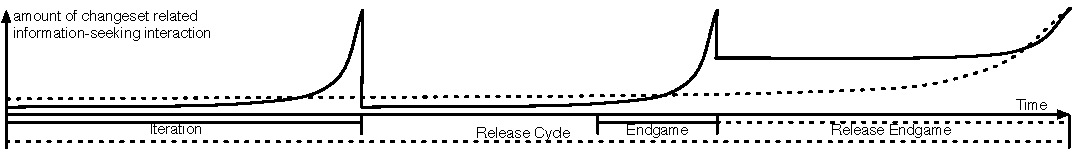
\includegraphics[width=\textwidth]{figures/findingProcess2}
\vspace{-20pt}\caption{The pattern of information-seeking interactions throughout several iterations of a release cycle. Every release cycle consists of a number of iterations; each iteration includes an endgame phase. Changeset-based interactions are more frequent during endgame phases and during the last iteration of the release cycle.}
\label{IterationsFig}
\end{figure}



\begin{table}[t!]
\centering
\begin{tabular}{rll}
\toprule
%\vspace{-2pt} Process-related items\\
%\midrule
Process-related items &\vspace{-2pt}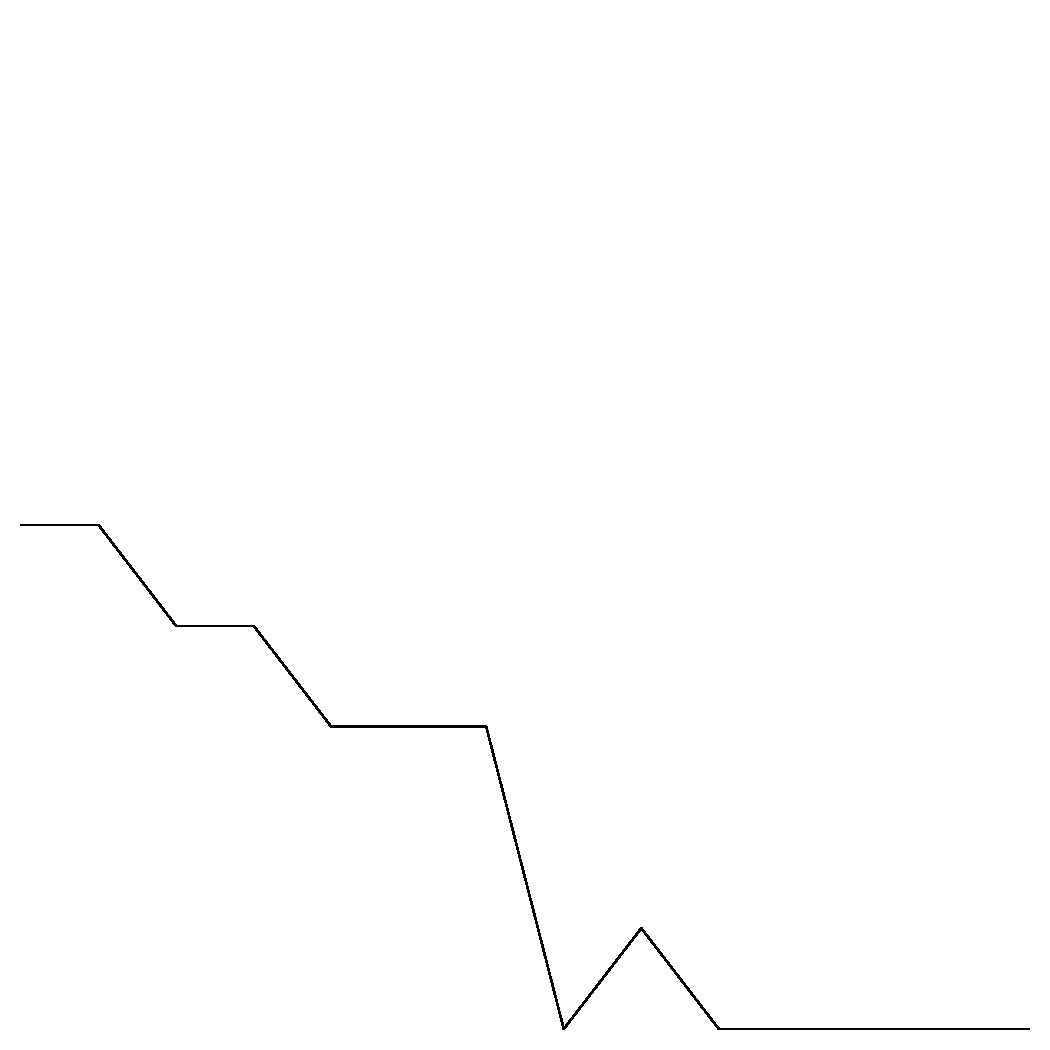
\includegraphics[height=10px, width=30px]{figures/sparkles/during-release-endgame.pdf} & Release endgame\\
&\vspace{-2pt}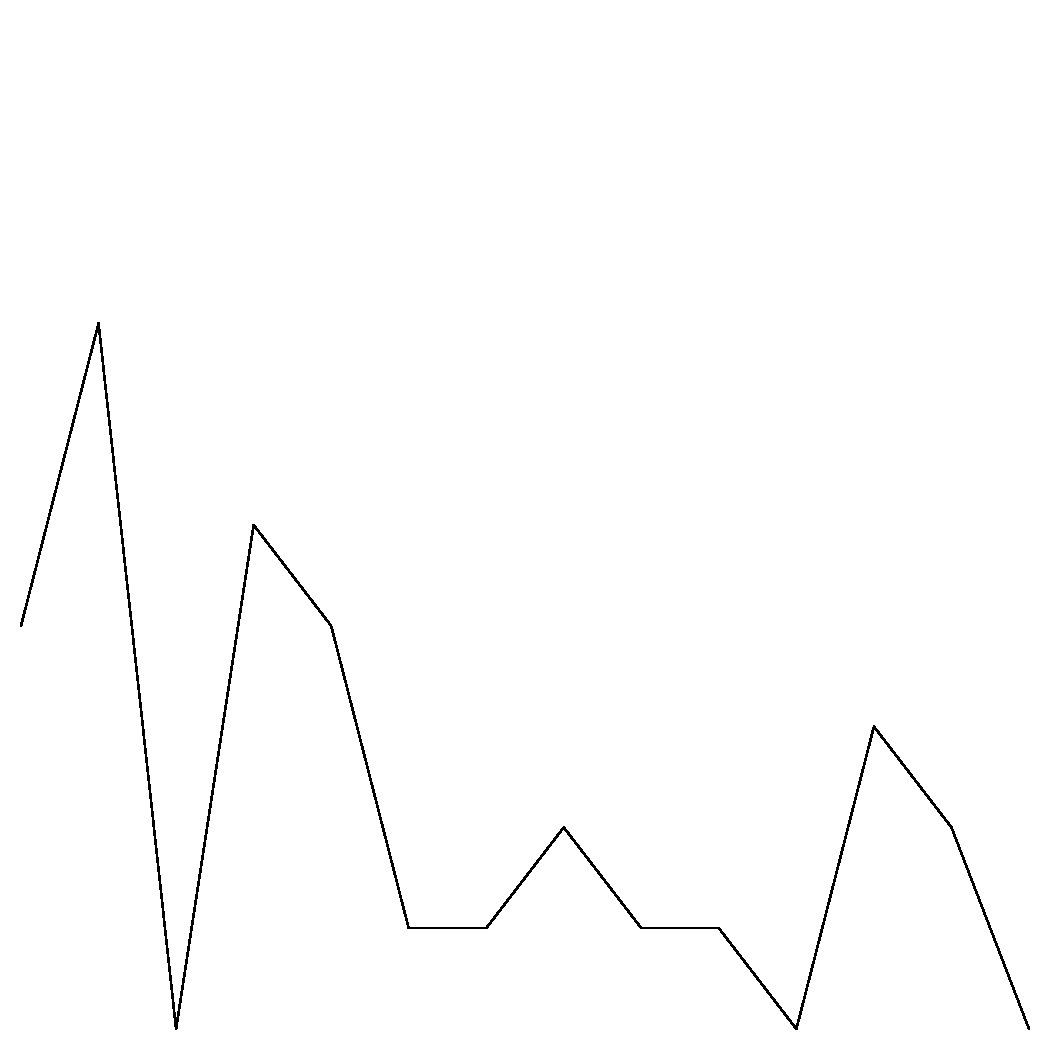
\includegraphics[height=10px, width=30px]{figures/sparkles/you-need-to-review-a-change.pdf} & To review the change\\
&\vspace{-2pt}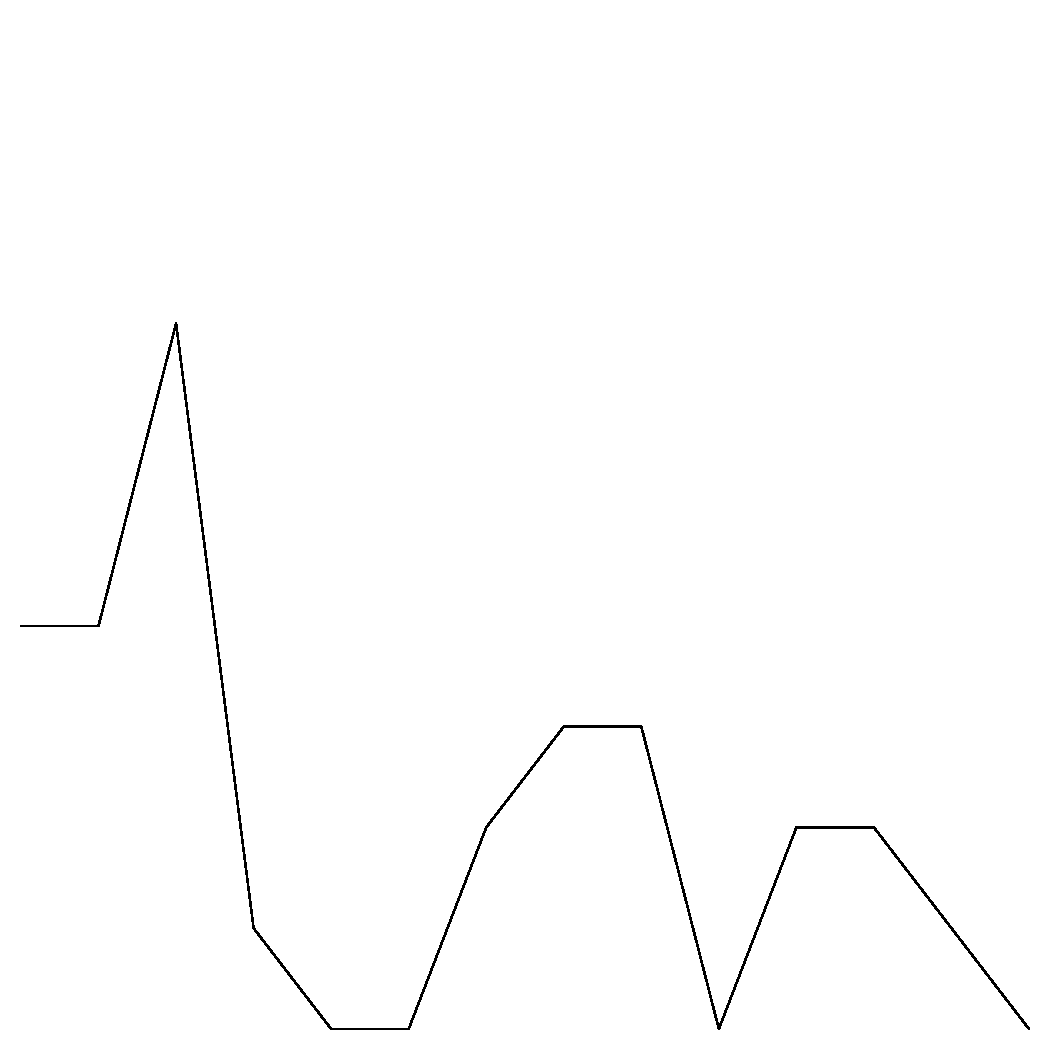
\includegraphics[height=10px, width=30px]{figures/sparkles/you-need-to-approve-a-change.pdf} & To approve the change\\
&\vspace{-2pt}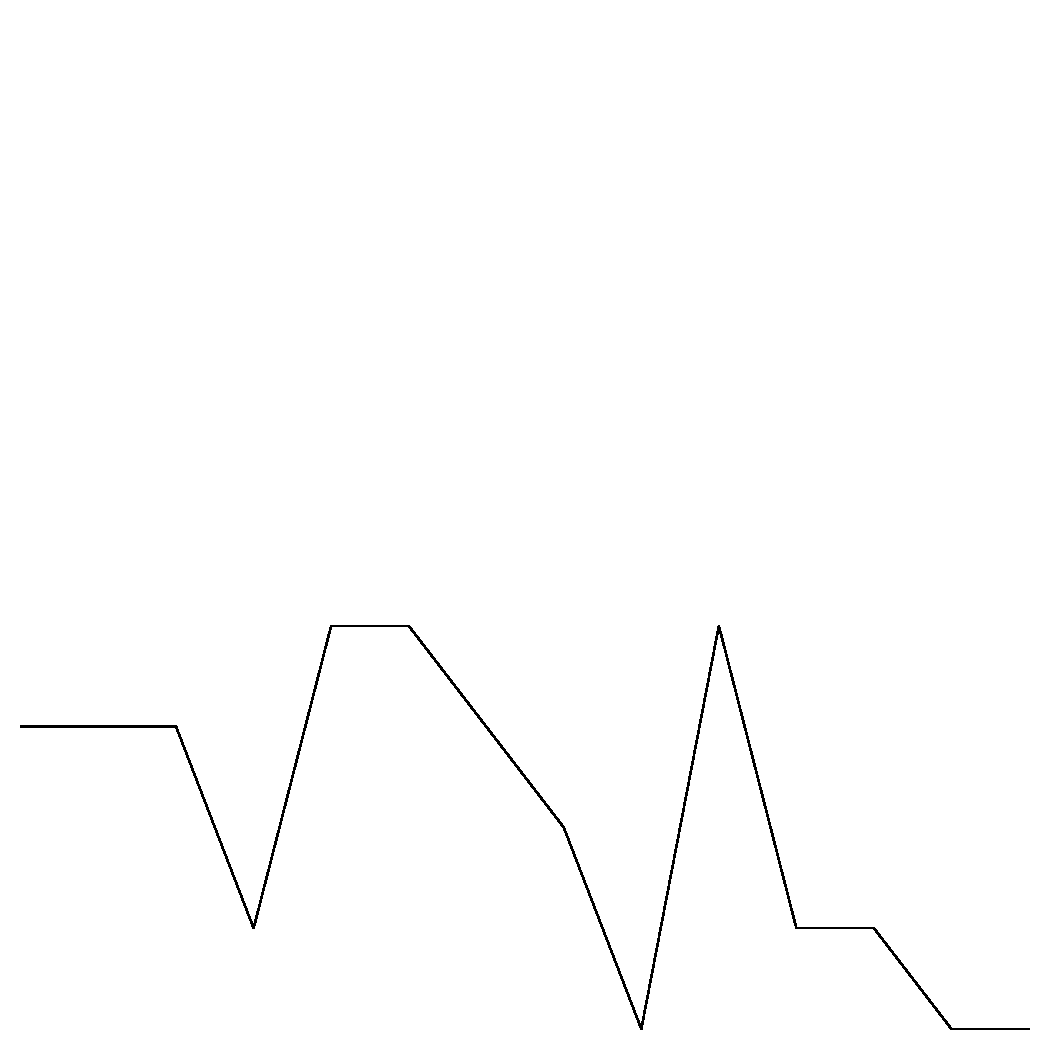
\includegraphics[height=10px, width=30px]{figures/sparkles/late-milestone.pdf} & Late milestone\\
&\vspace{-2pt}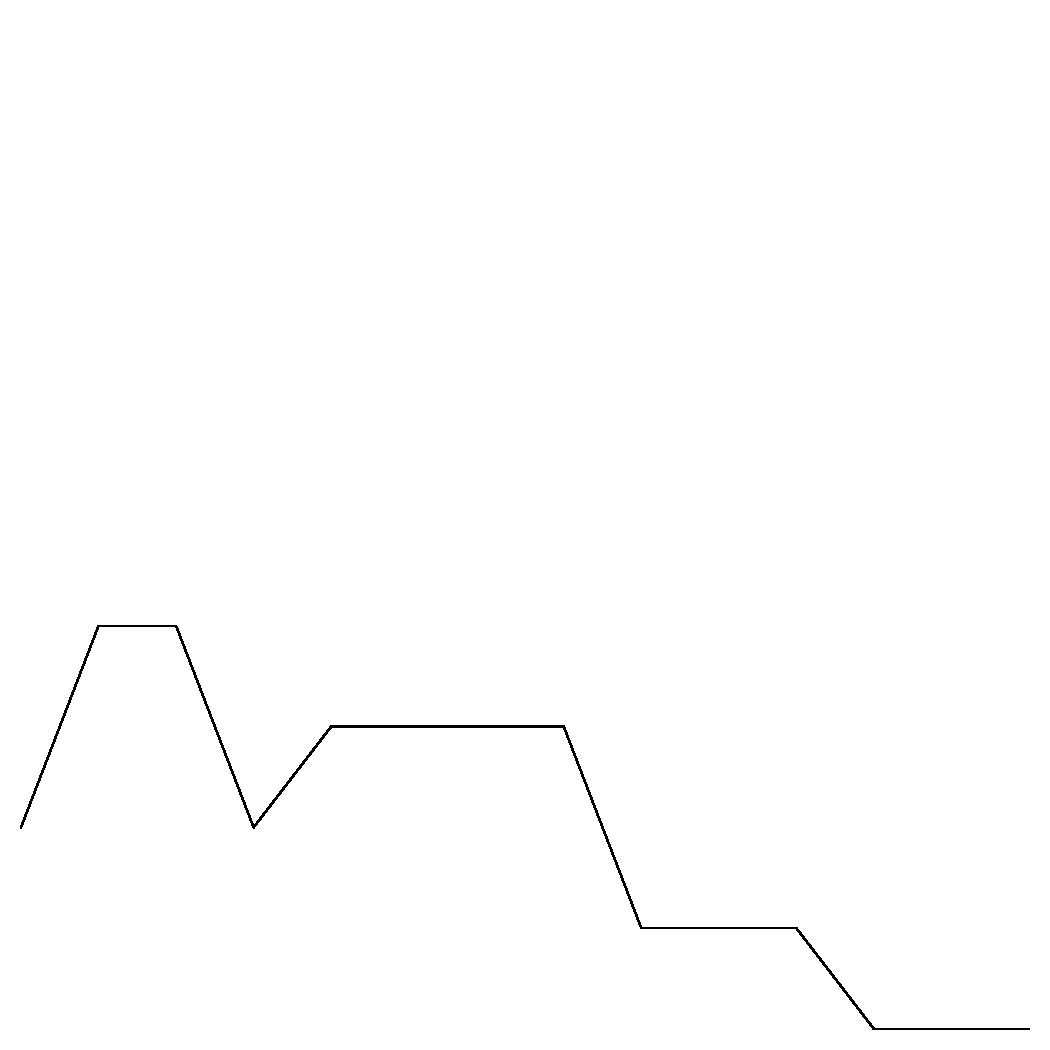
\includegraphics[height=10px, width=30px]{figures/sparkles/during-iteration-endgame.pdf} & During iteration endgame\\
&\vspace{-2pt}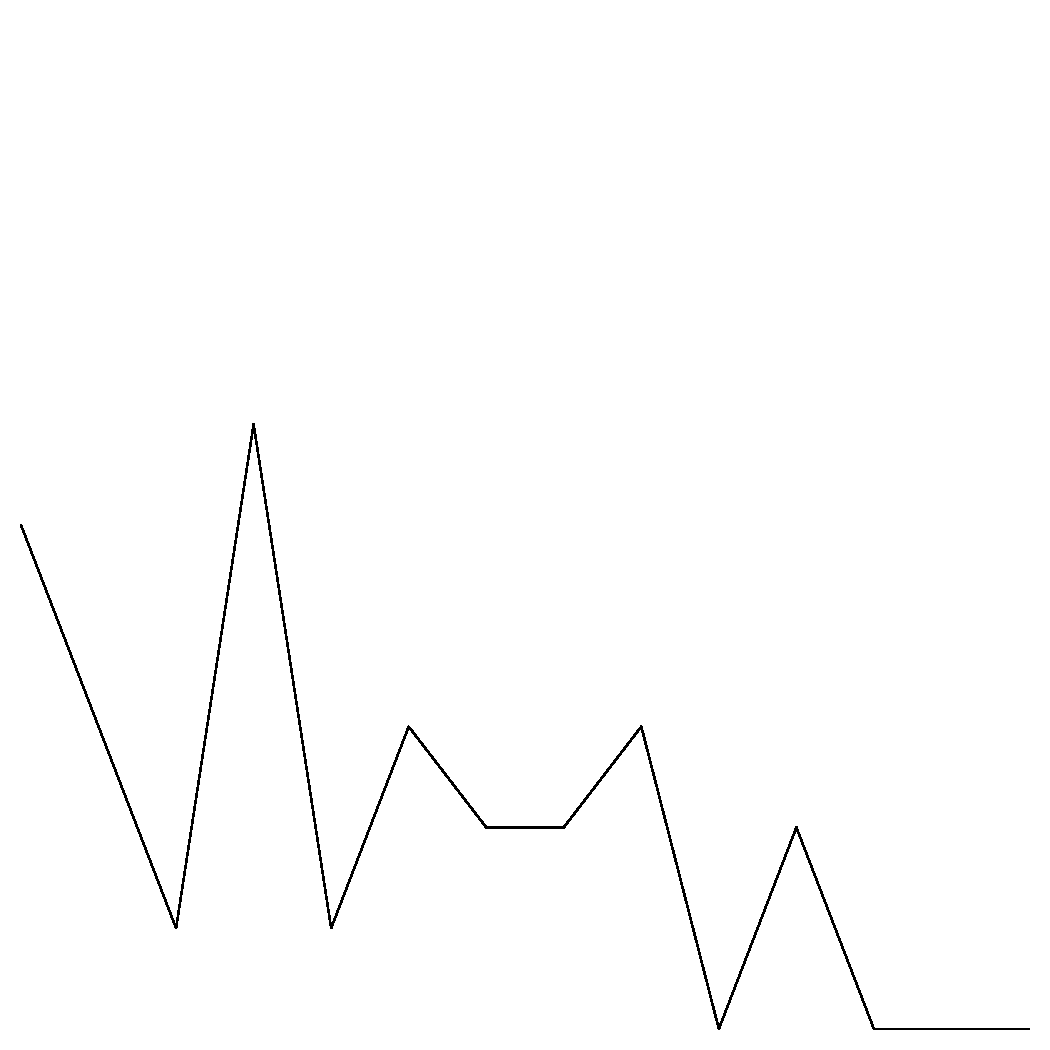
\includegraphics[height=10px, width=30px]{figures/sparkles/you-need-a-review-for-a-change.pdf} & Obtain a review for the change\\
&\vspace{-2pt}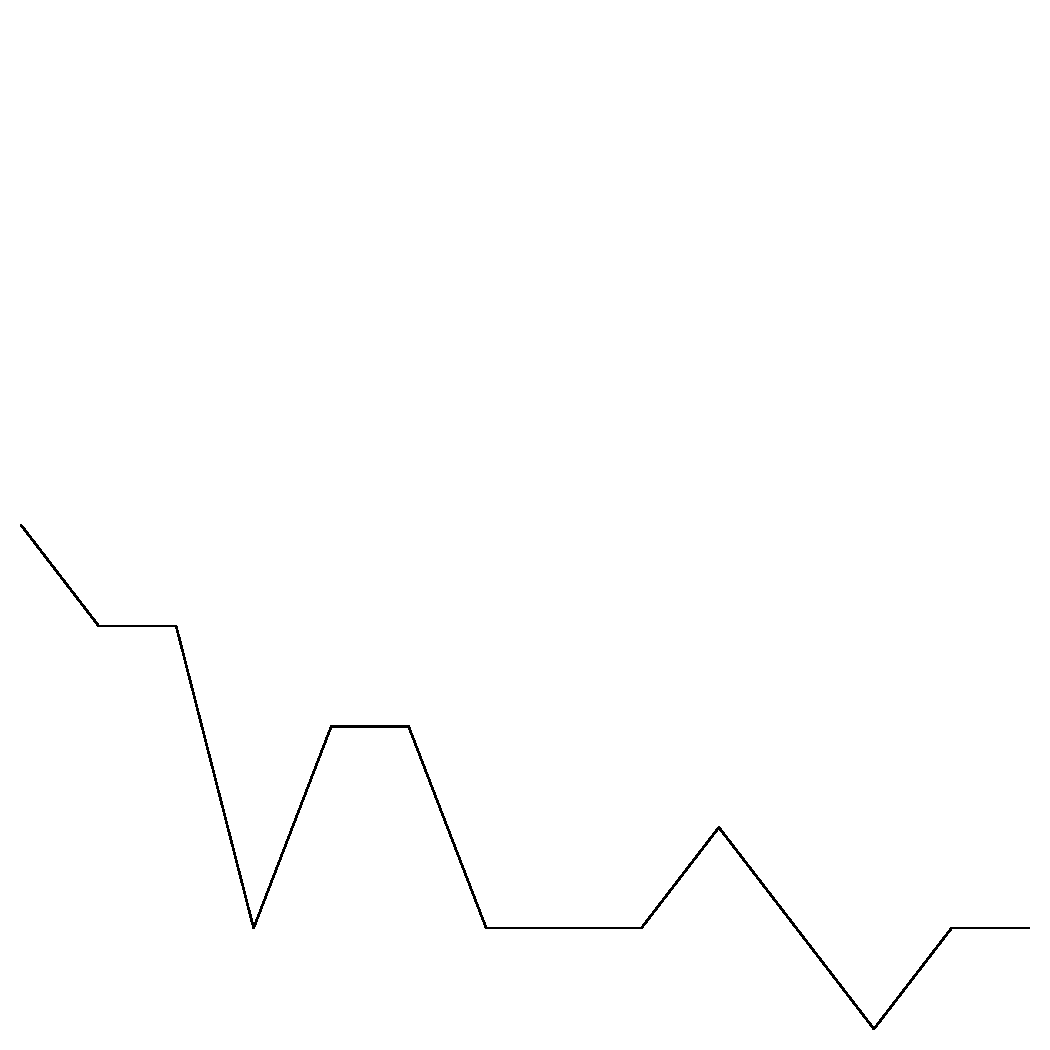
\includegraphics[height=10px, width=30px]{figures/sparkles/you-need-an-approval-for-a-change.pdf} & Obtain an approval for the change\\
&\vspace{-2pt}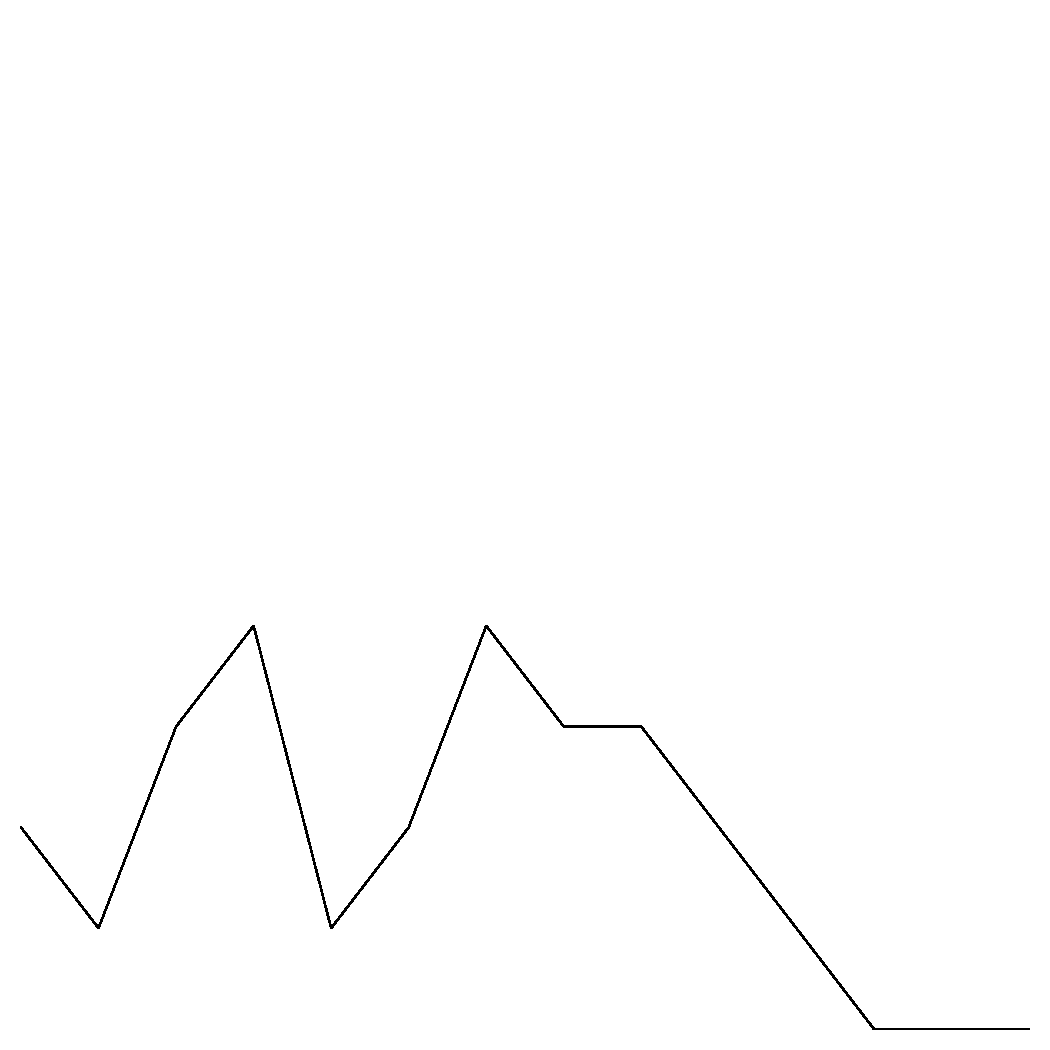
\includegraphics[height=10px, width=30px]{figures/sparkles/related-work-item-has-high-severity.pdf} & Related work item has high severity\\
&\vspace{-2pt}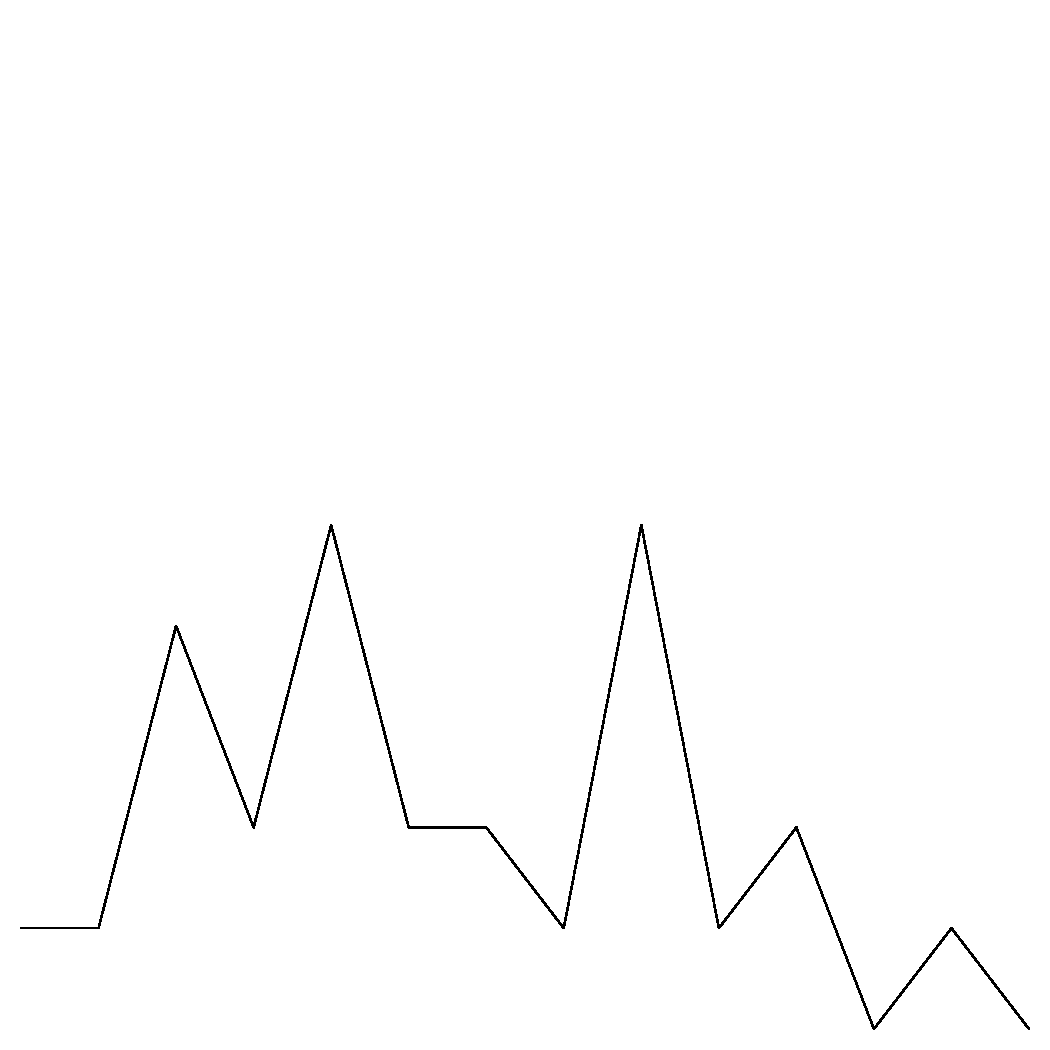
\includegraphics[height=10px, width=30px]{figures/sparkles/you-need-to-verify-a-fix.pdf} & Verify a fix\\
&\vspace{-2pt}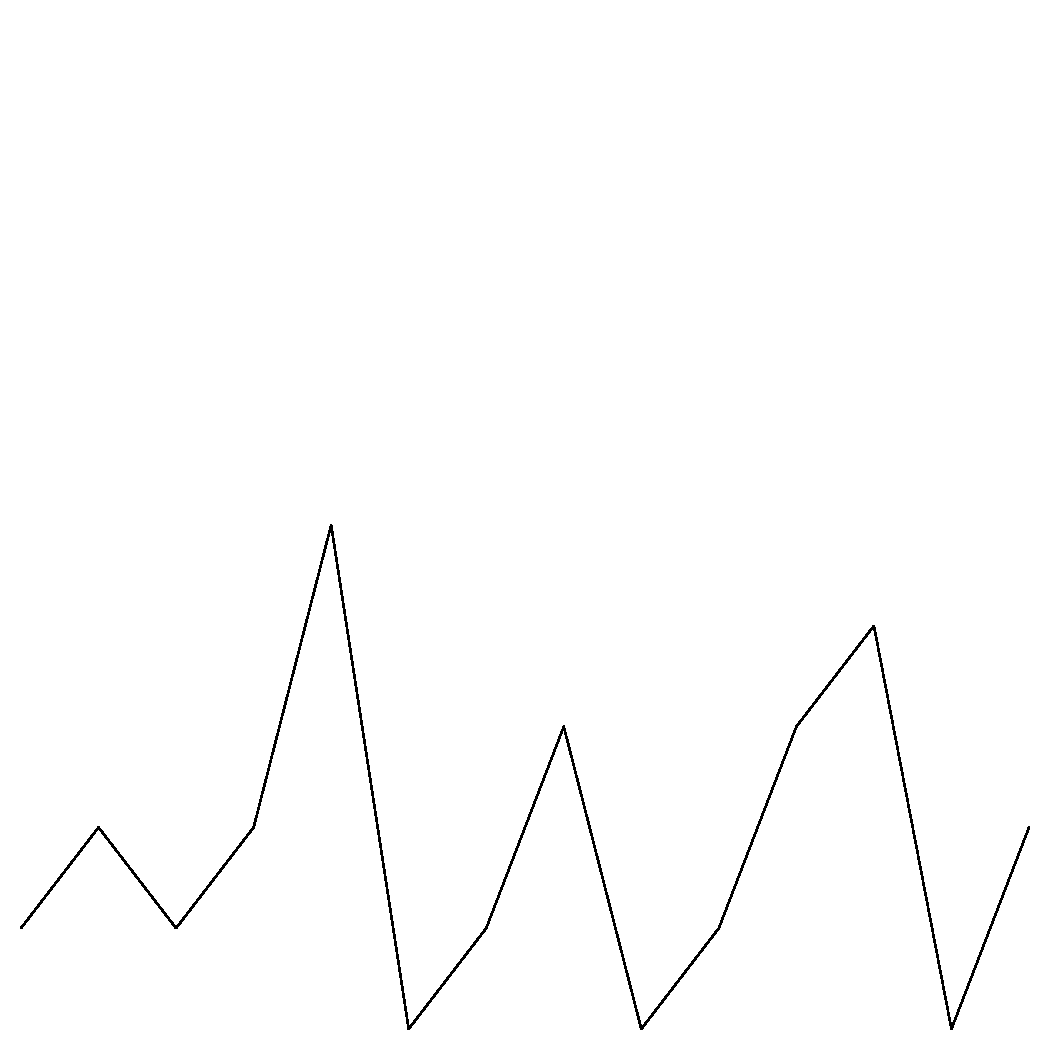
\includegraphics[height=10px, width=30px]{figures/sparkles/topic-of-work-item-the-change-is-attached-to.pdf} & Topic of work item the change is attached to\\ 
&\vspace{-2pt}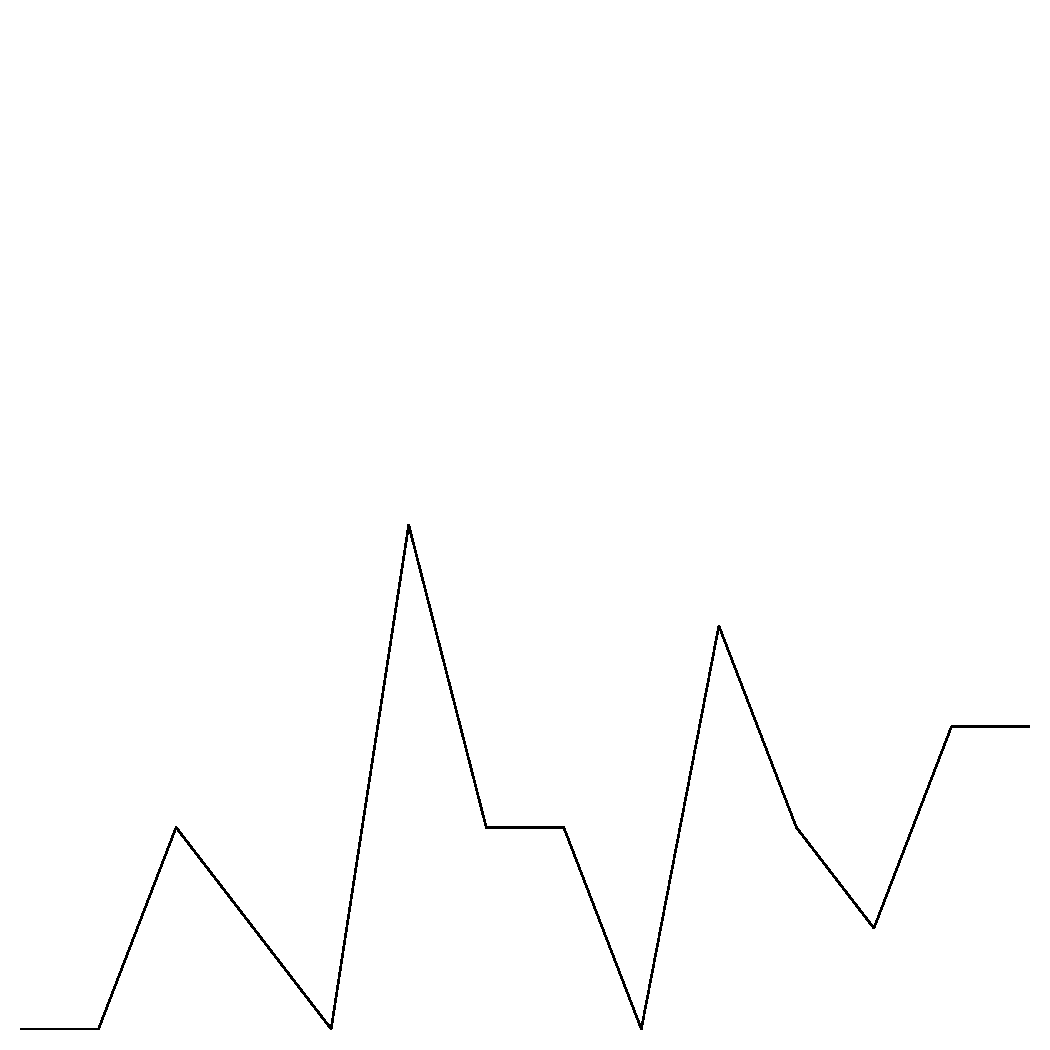
\includegraphics[height=10px, width=30px]{figures/sparkles/priority-of-related-work-item-was-set-from-your-team-lead.pdf} & Priority set by your team lead\\
&\vspace{-2pt}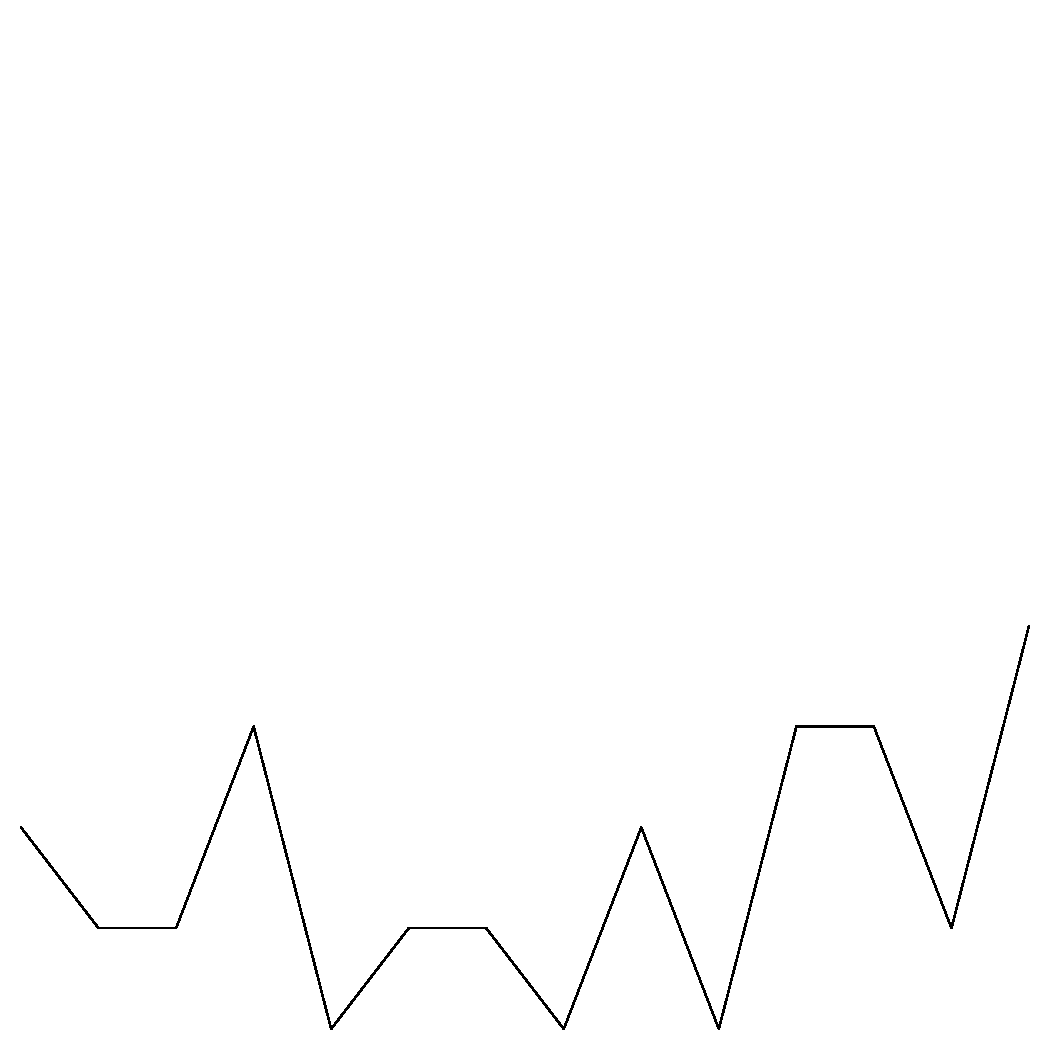
\includegraphics[height=10px, width=30px]{figures/sparkles/role-of-committer--e-g--developer--team-lead--intern.pdf} & Role of the committer (e.g. developer)\\
&\vspace{-2pt}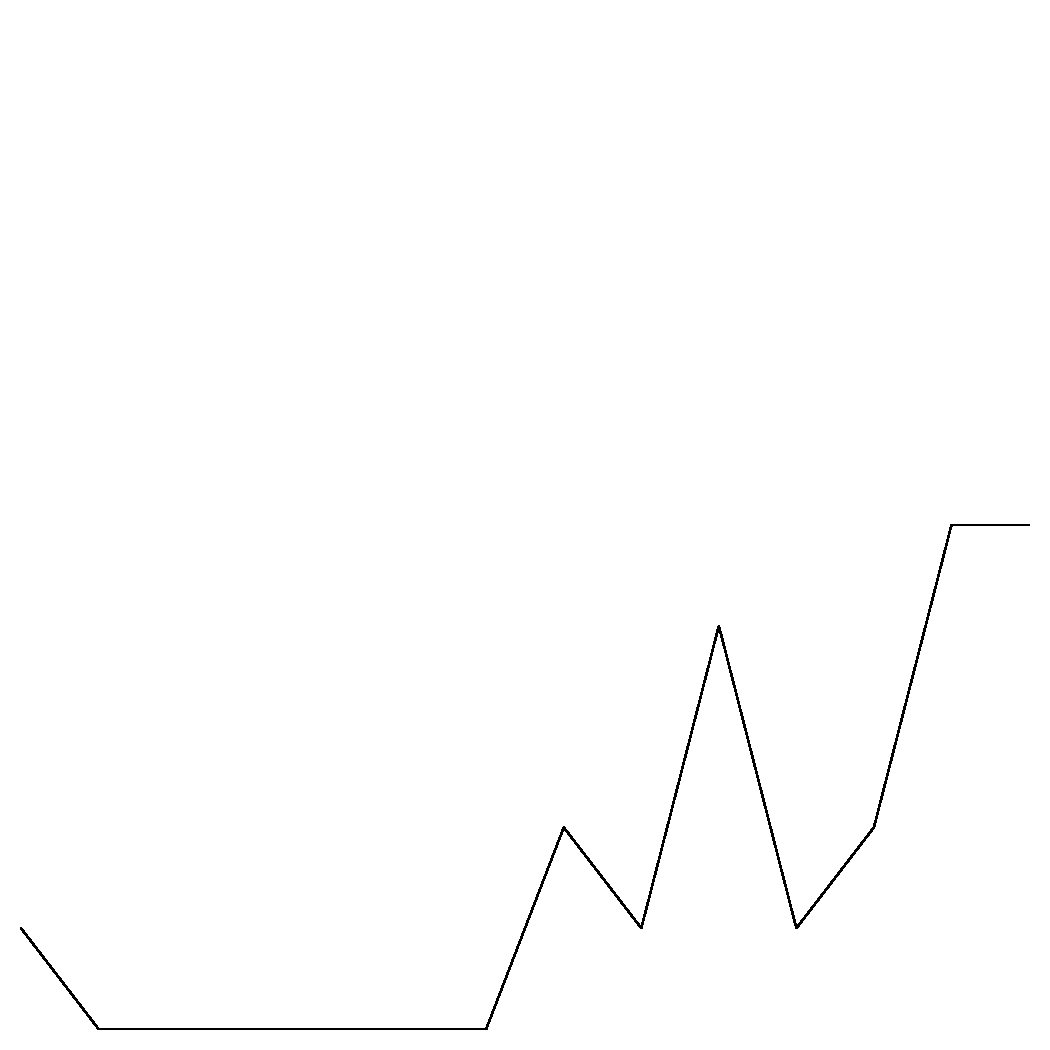
\includegraphics[height=10px, width=30px]{figures/sparkles/early-in-an-iteration.pdf} & Early in an iteration\\
&\vspace{-2pt}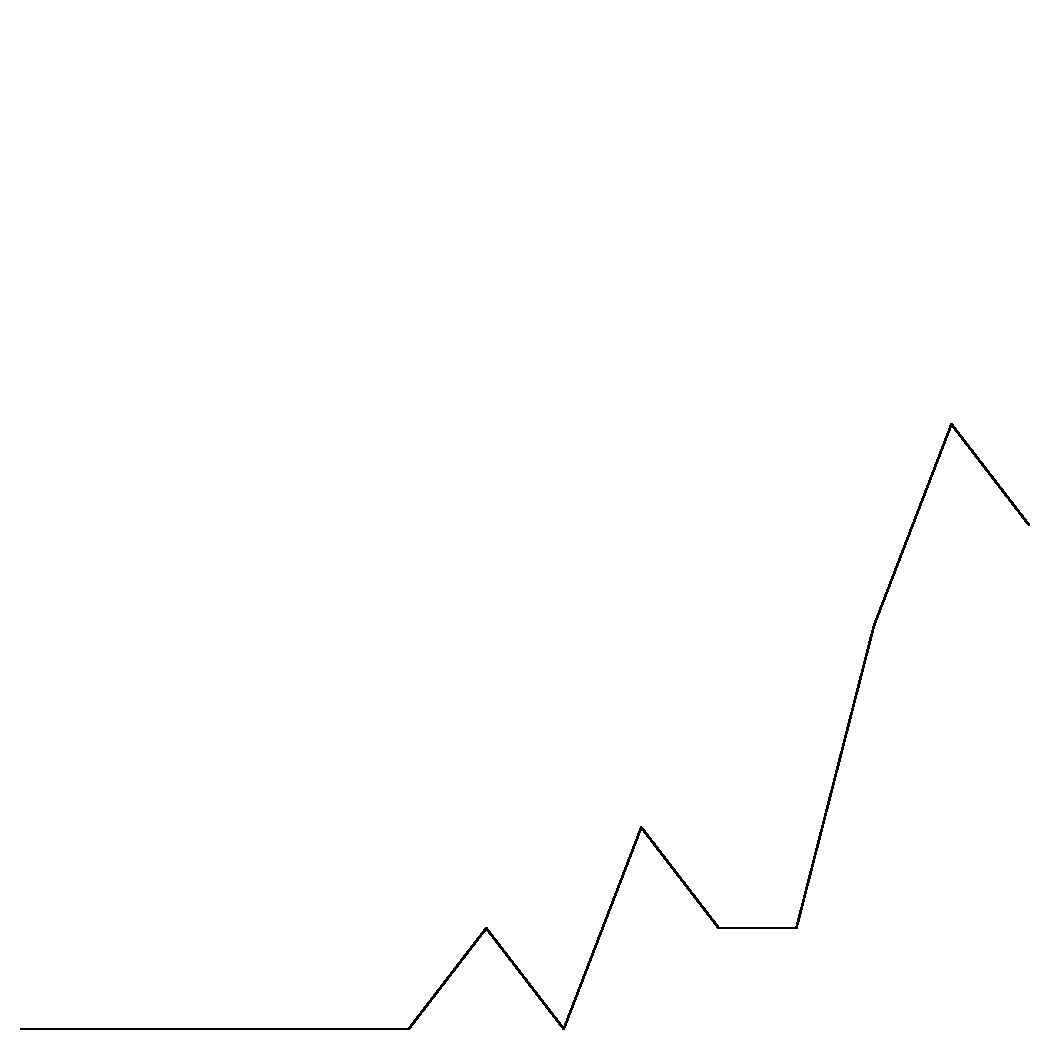
\includegraphics[height=10px, width=30px]{figures/sparkles/early-milestone.pdf} & Early milestone\\
\midrule
%\vspace{-2pt}& Developer-related items\\
%\midrule
Developer-related items&\vspace{-2pt}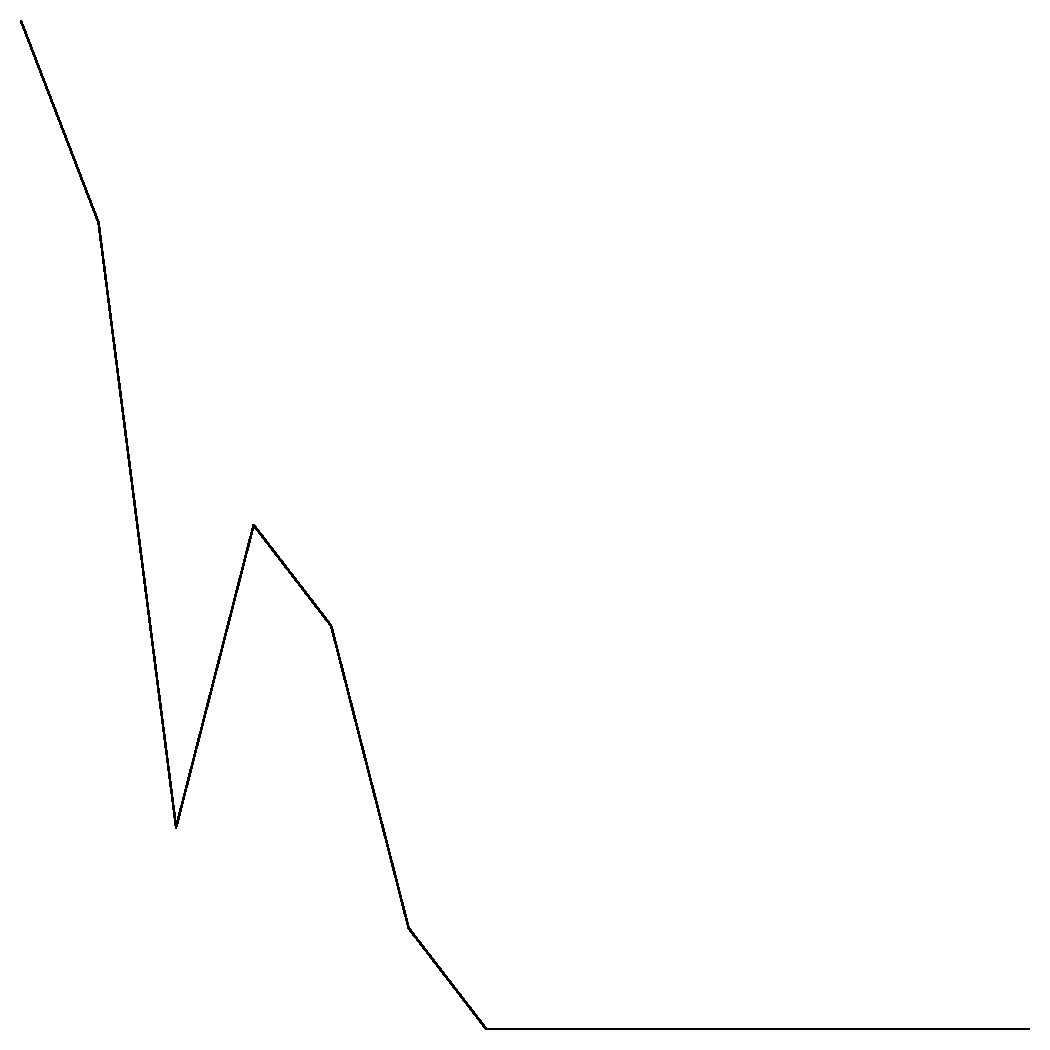
\includegraphics[height=10px, width=30px]{figures/sparkles/change-author-is-inexperienced.pdf} & Author is inexperienced\\
&\vspace{-2pt}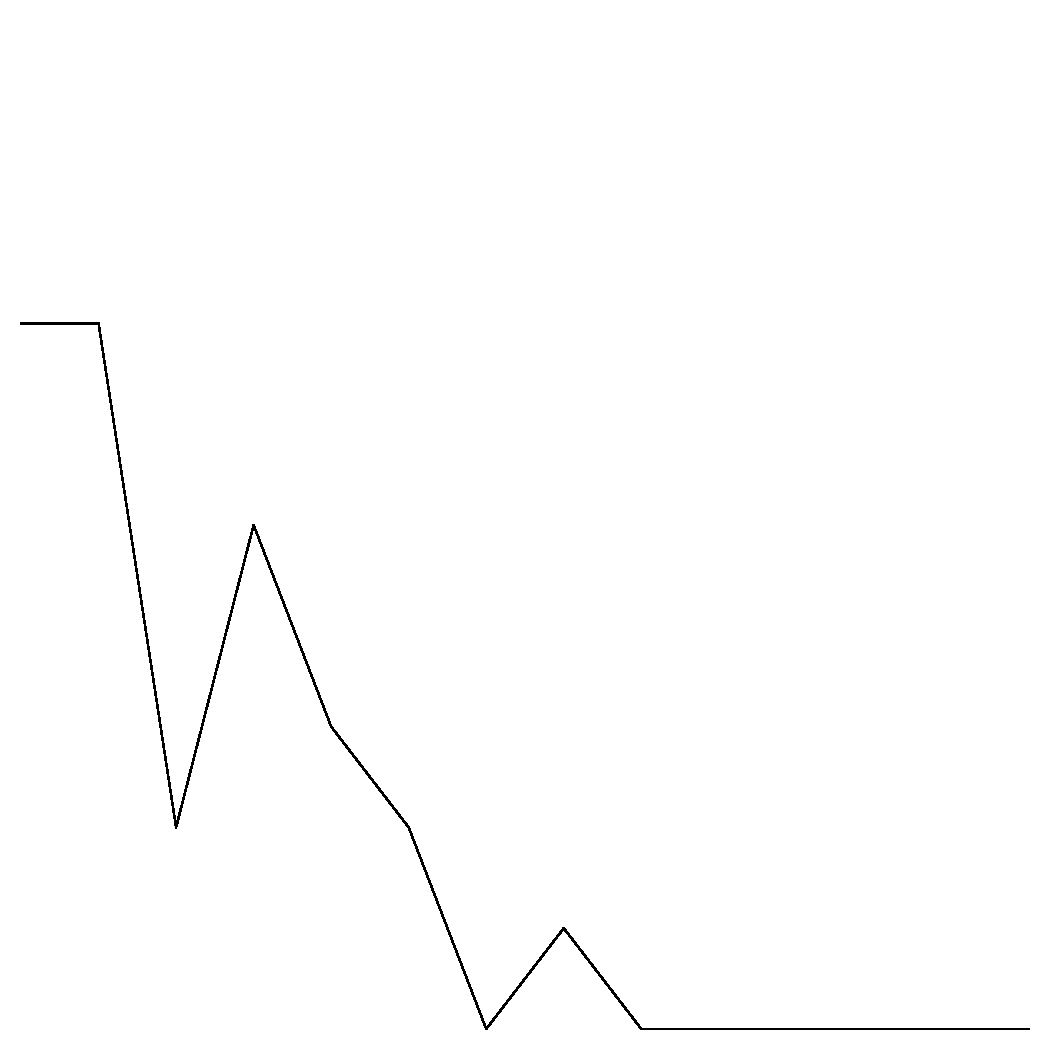
\includegraphics[height=10px, width=30px]{figures/sparkles/recent-work-of-low-quality.pdf} & Author recently delivered sub-standard work\\
&\vspace{-2pt}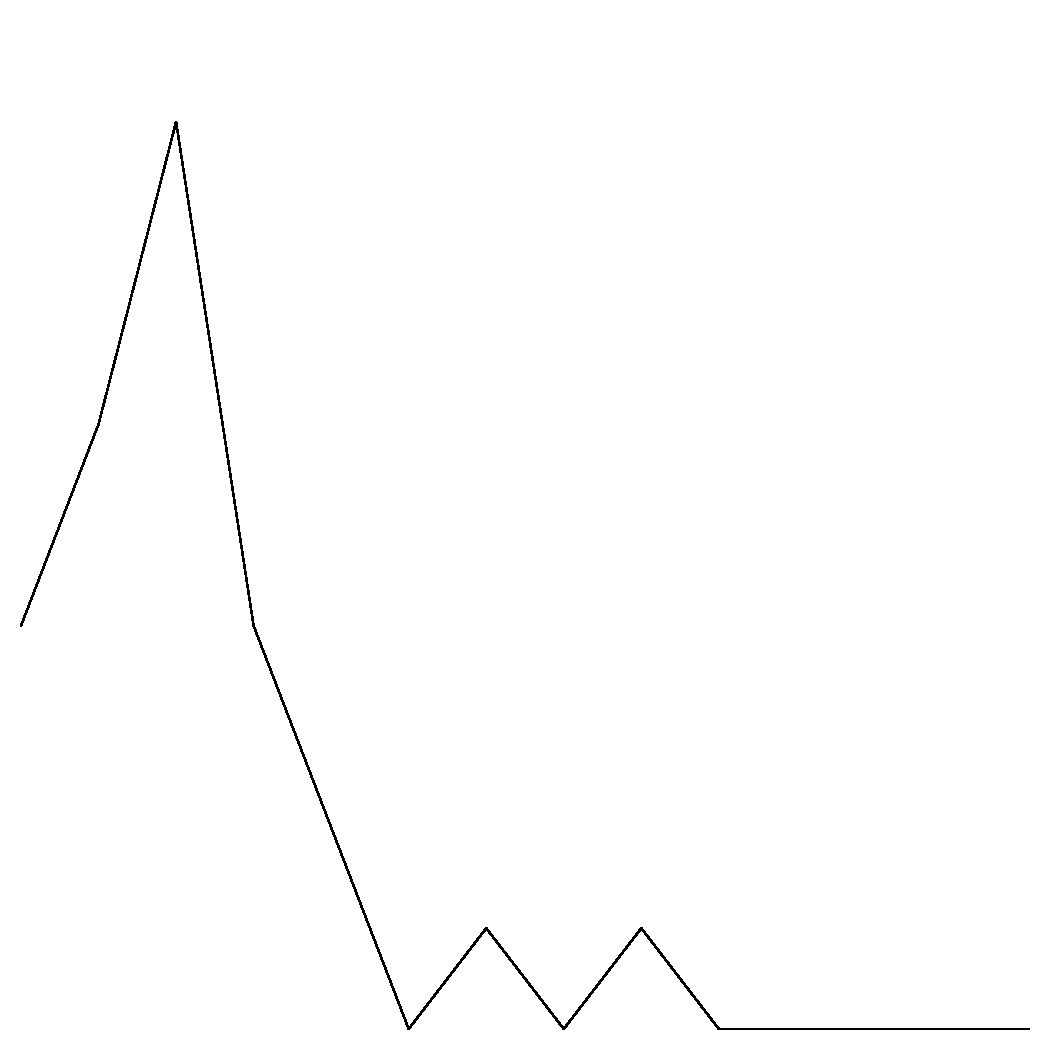
\includegraphics[height=10px, width=30px]{figures/sparkles/change-author-is-not-up-to-date-with-recent-events.pdf} & Author is not up to date with recent events\\
&\vspace{-2pt}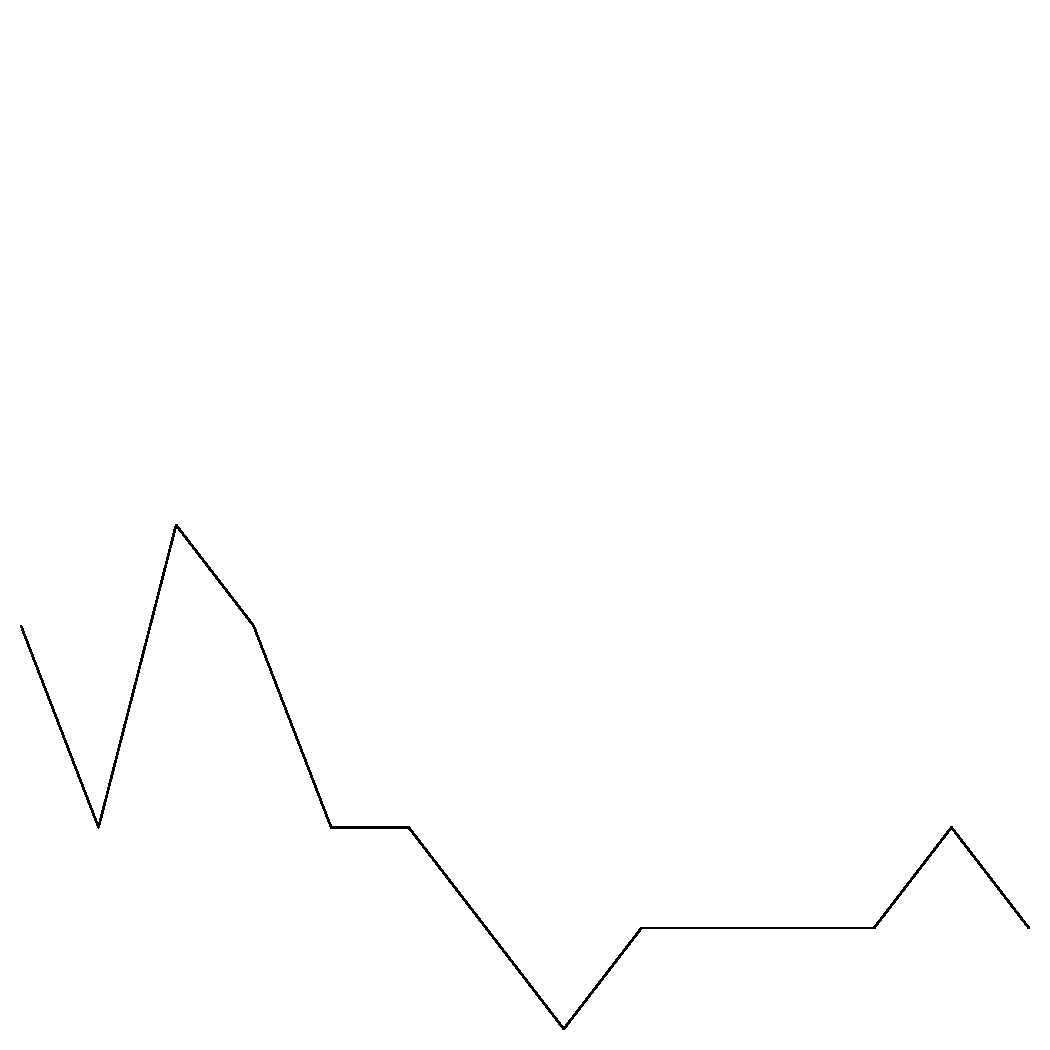
\includegraphics[height=10px, width=30px]{figures/sparkles/don-t-know-the-change-author.pdf} & You do not know the change-set author \\
&\vspace{-2pt}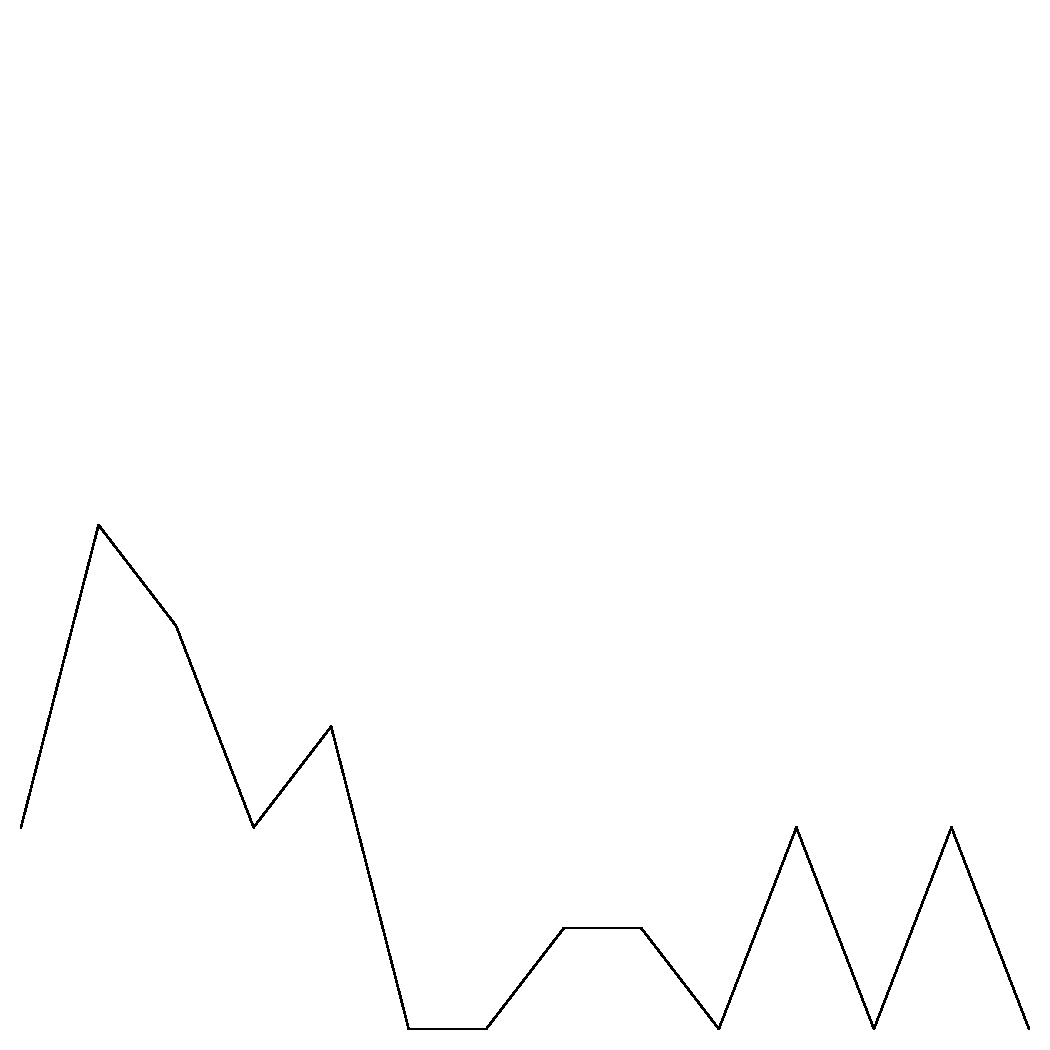
\includegraphics[height=10px, width=30px]{figures/sparkles/currently-working-with-the-change-author.pdf} & Author is currently working with you\\
&\vspace{-2pt}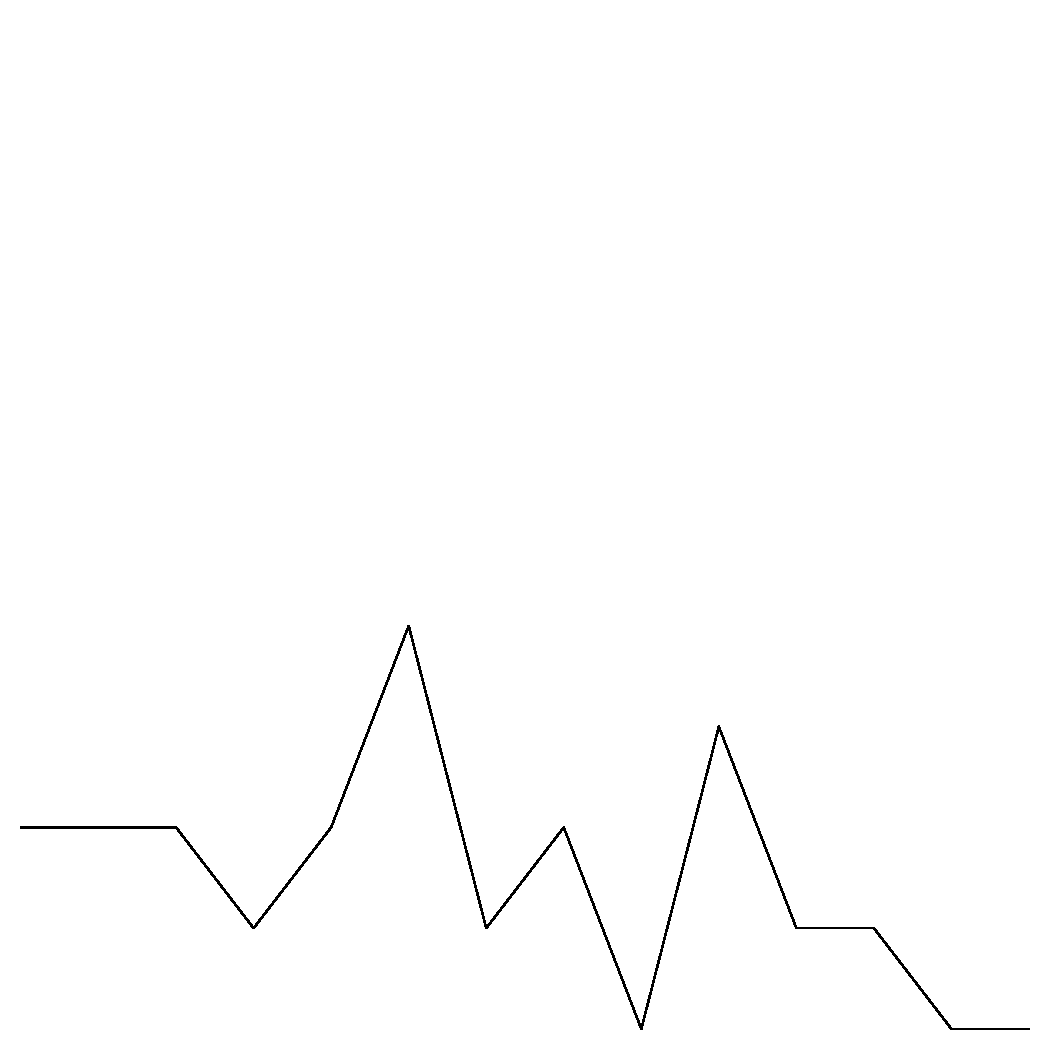
\includegraphics[height=10px, width=30px]{figures/sparkles/change-author-part-of-the-same-feature-team.pdf} & Author part of same feature team\\
&\vspace{-2pt}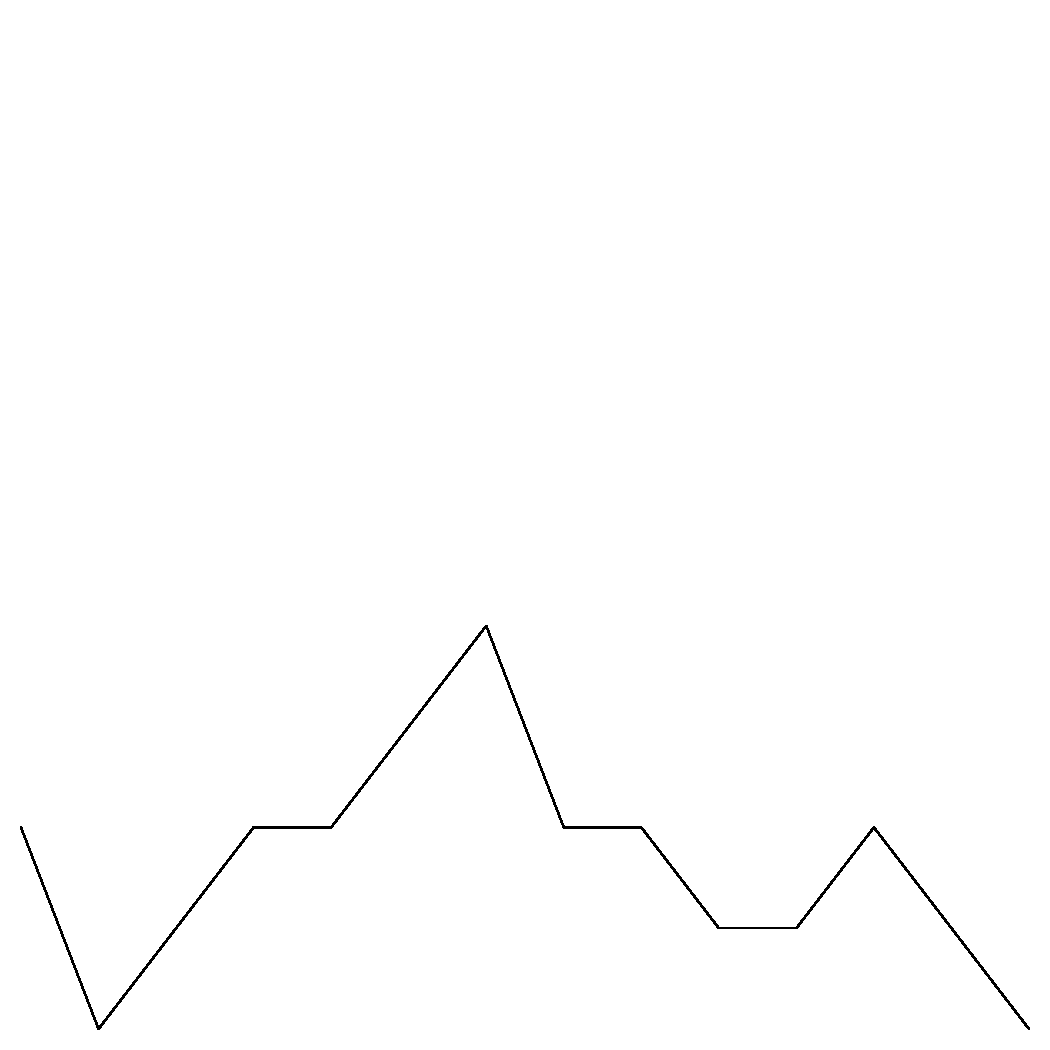
\includegraphics[height=10px, width=30px]{figures/sparkles/team-of-change-author.pdf} & Author part of your team\\
&\vspace{-2pt}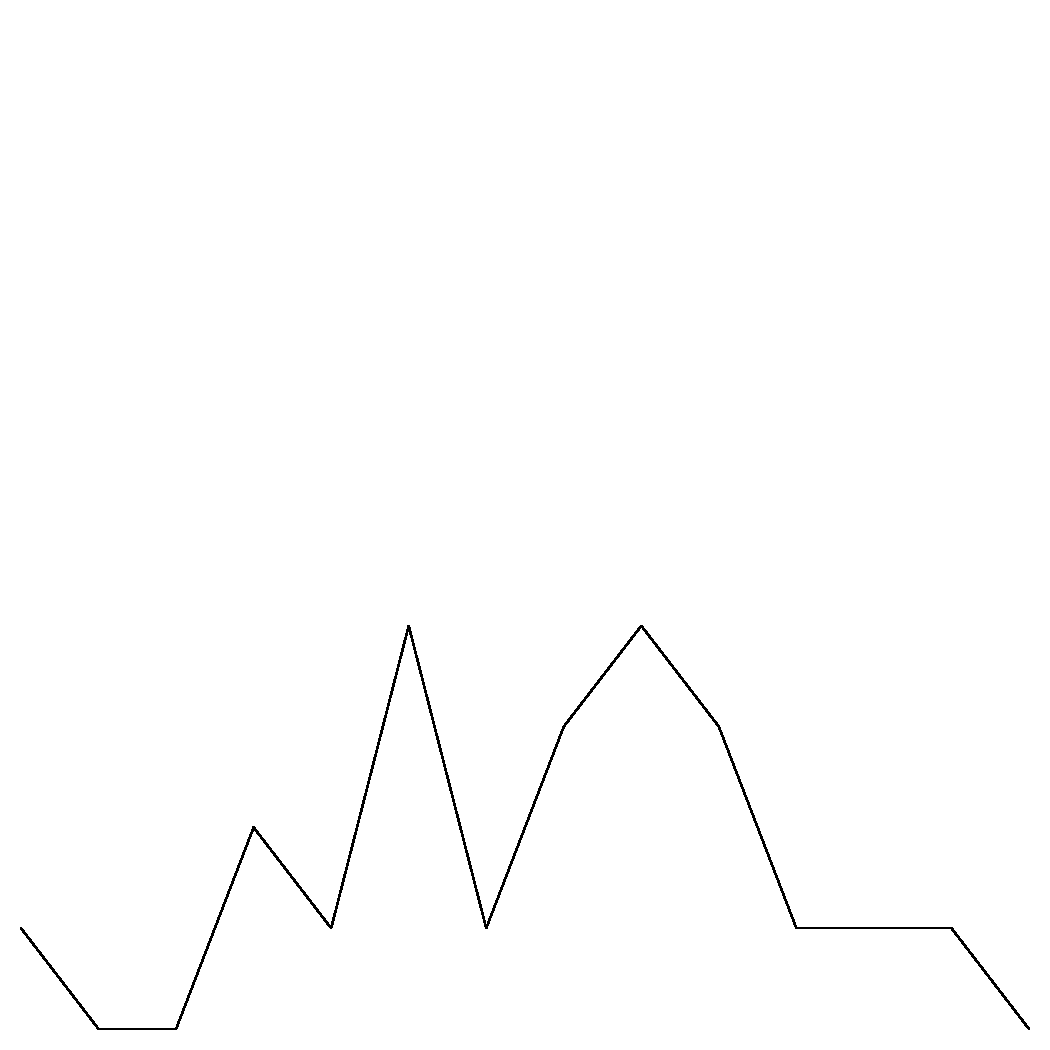
\includegraphics[height=10px, width=30px]{figures/sparkles/worked-with-change-author-in-the-past.pdf} & Worked with author before\\
&\vspace{-2pt}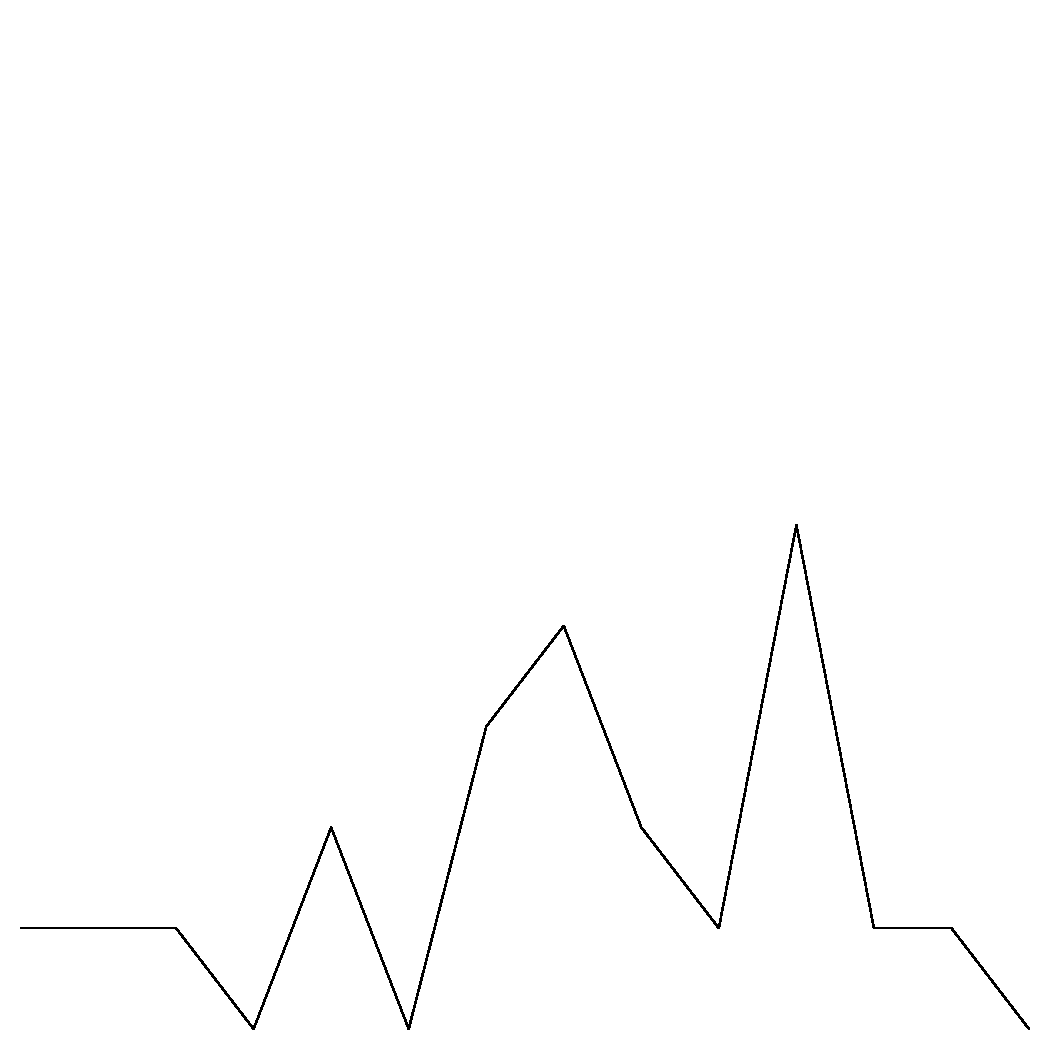
\includegraphics[height=10px, width=30px]{figures/sparkles/busyness-of-yourself} & Busyness of yourself\\
&\vspace{-2pt}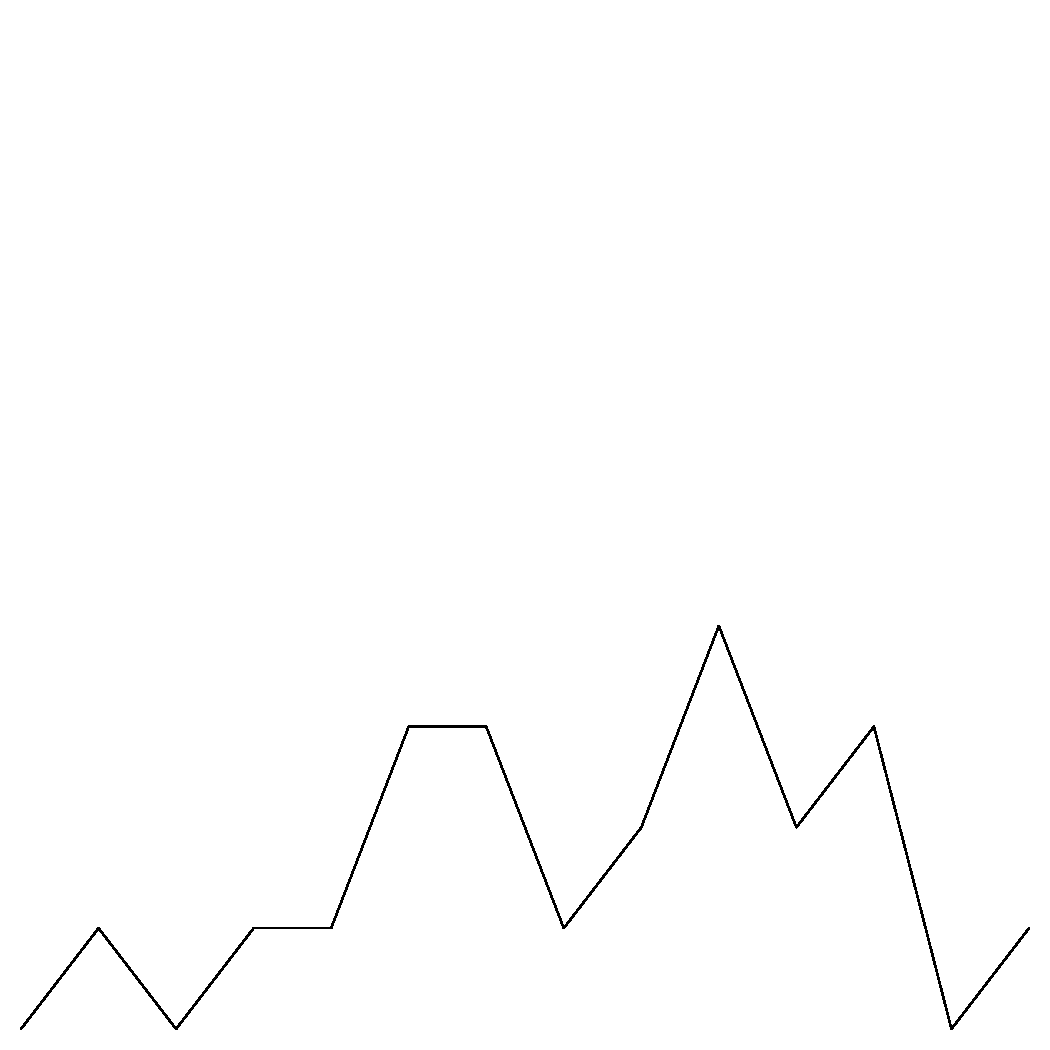
\includegraphics[height=10px, width=30px]{figures/sparkles/busyness-of-the-change-author} & Busyness of the author\\
&\vspace{-2pt}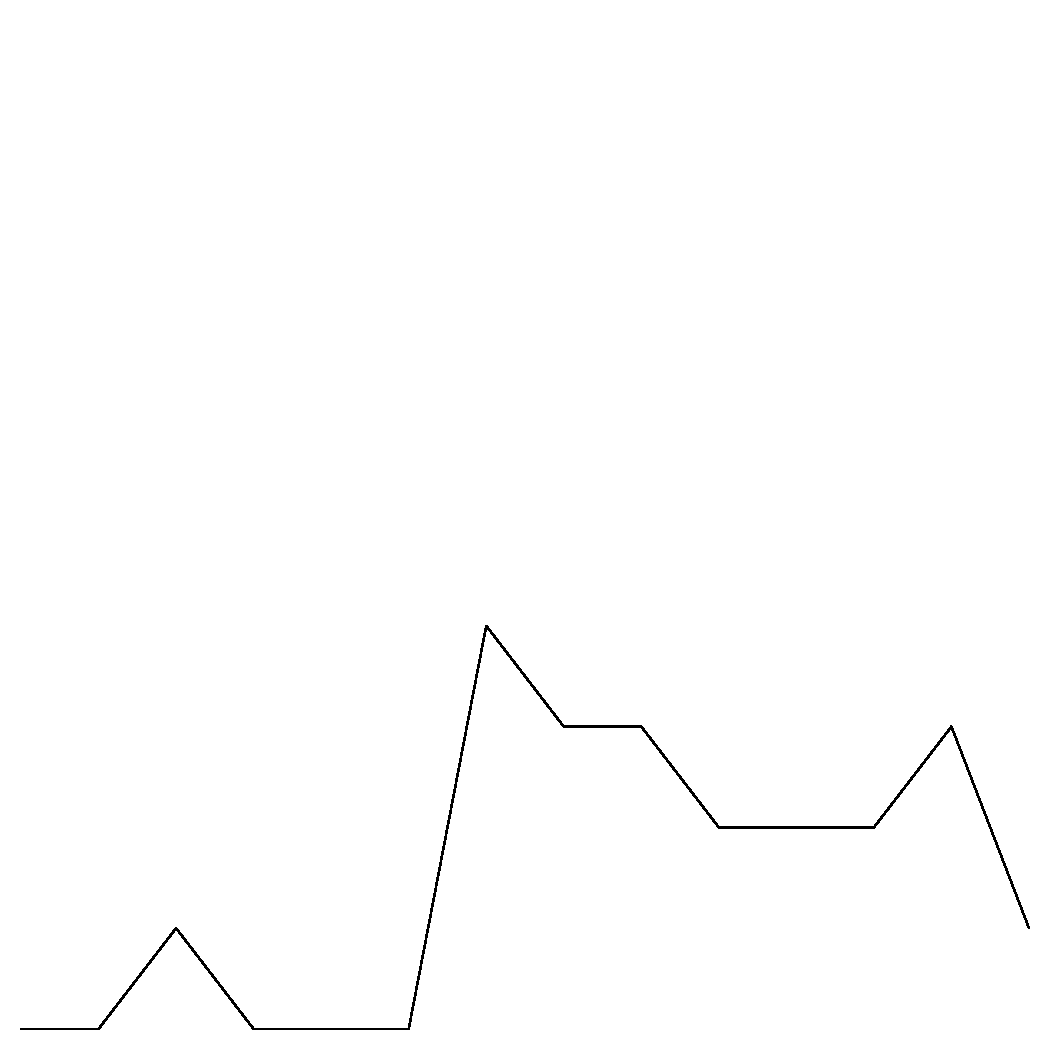
\includegraphics[height=10px, width=30px]{figures/sparkles/met-change-author-in-person.pdf} & Met in person\\
&\vspace{-2pt}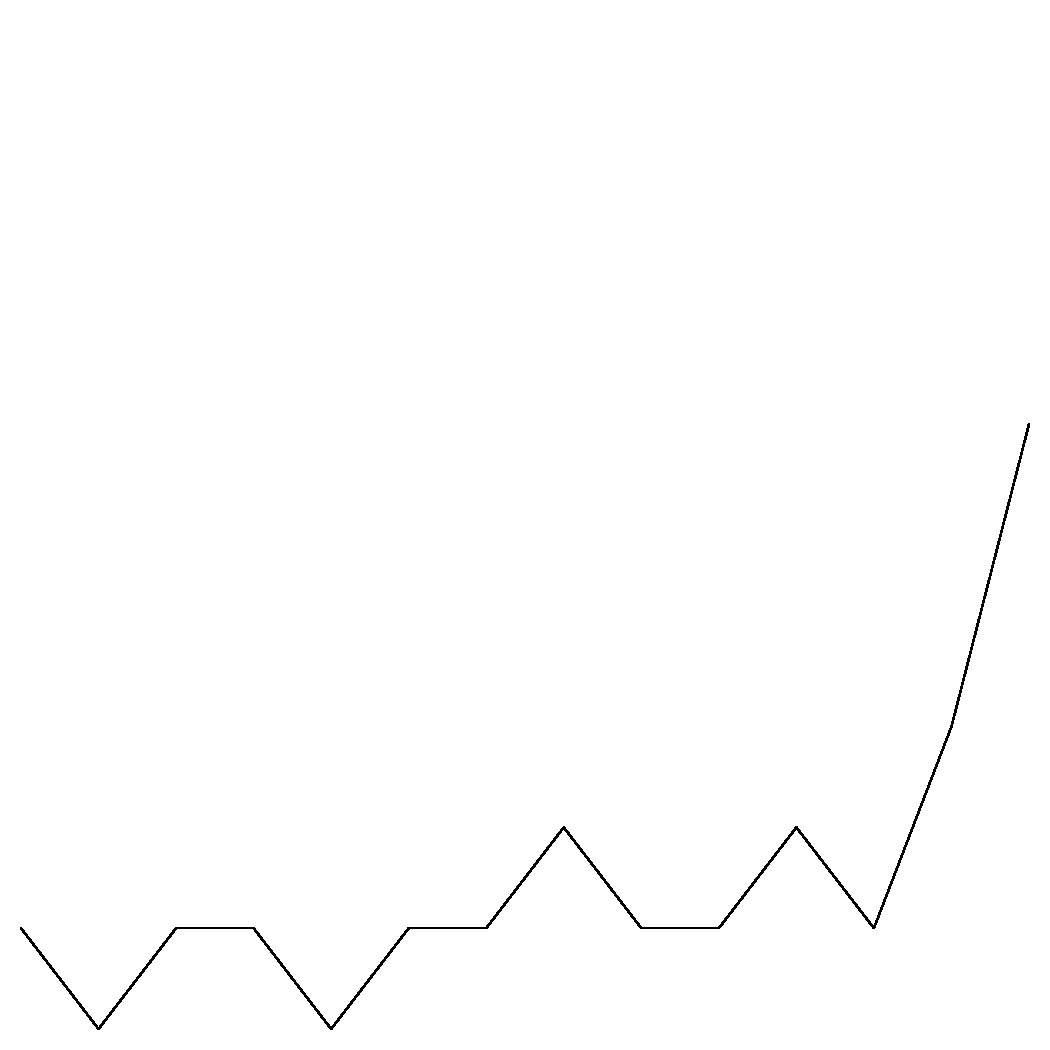
\includegraphics[height=10px, width=30px]{figures/sparkles/physical-location-of-the-change-author.pdf} & Physical location\\
&\vspace{-2pt}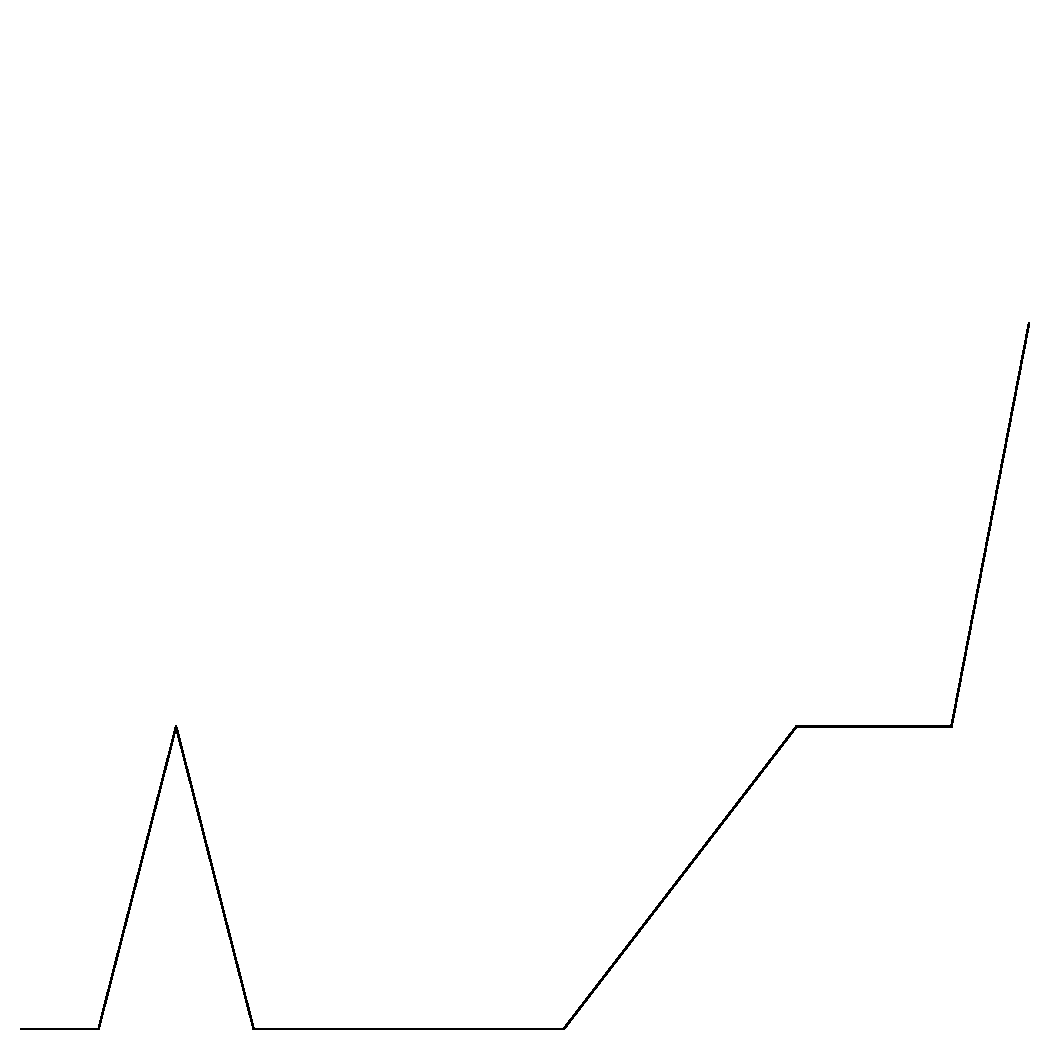
\includegraphics[height=10px, width=30px]{figures/sparkles/change-author-is-experienced.pdf} & Author is experienced\\
&\vspace{-2pt}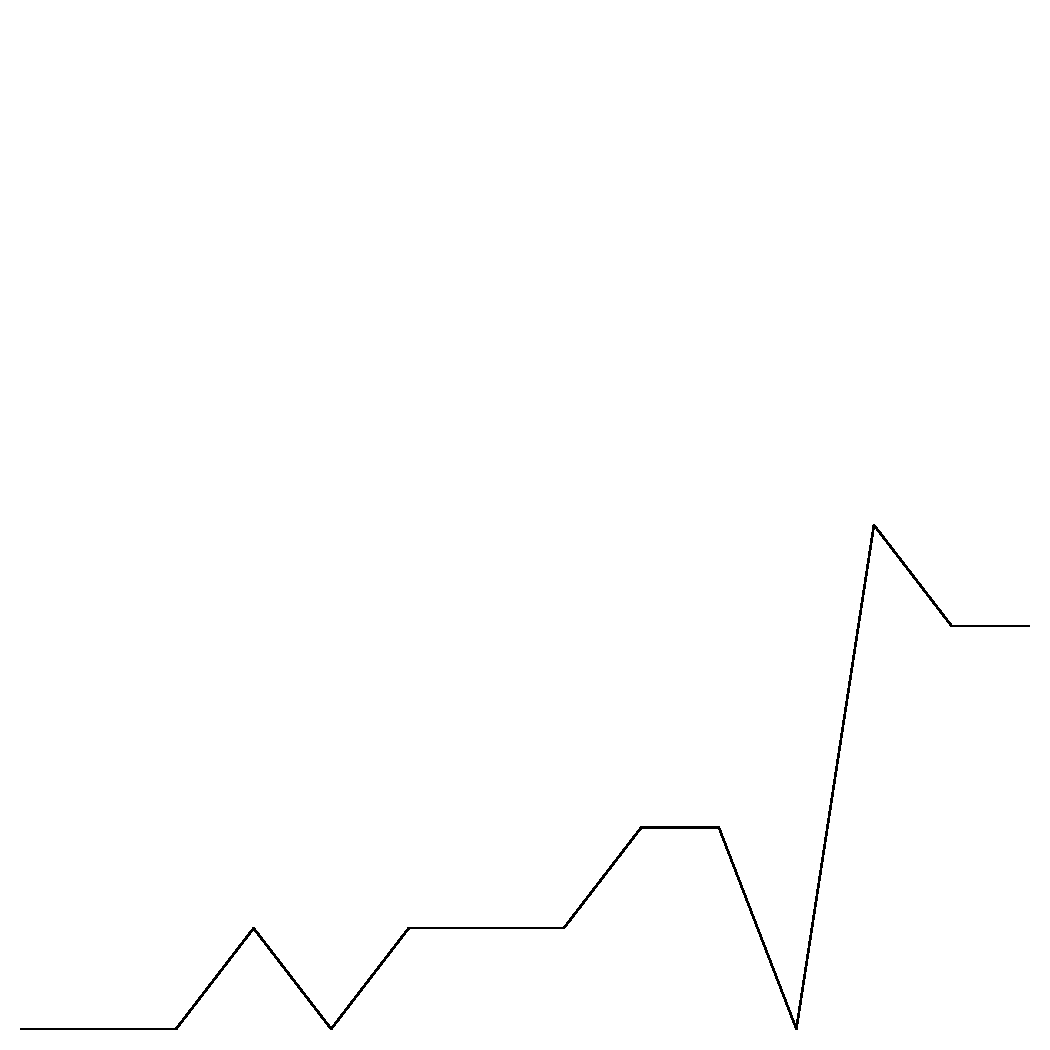
\includegraphics[height=10px, width=30px]{figures/sparkles/recent-work-of-high-quality.pdf} & Author recently delivered high-quality work\\
\midrule
%\vspace{-2pt}& Code-change related items \\
%\midrule
Code-change related items&\vspace{-2pt}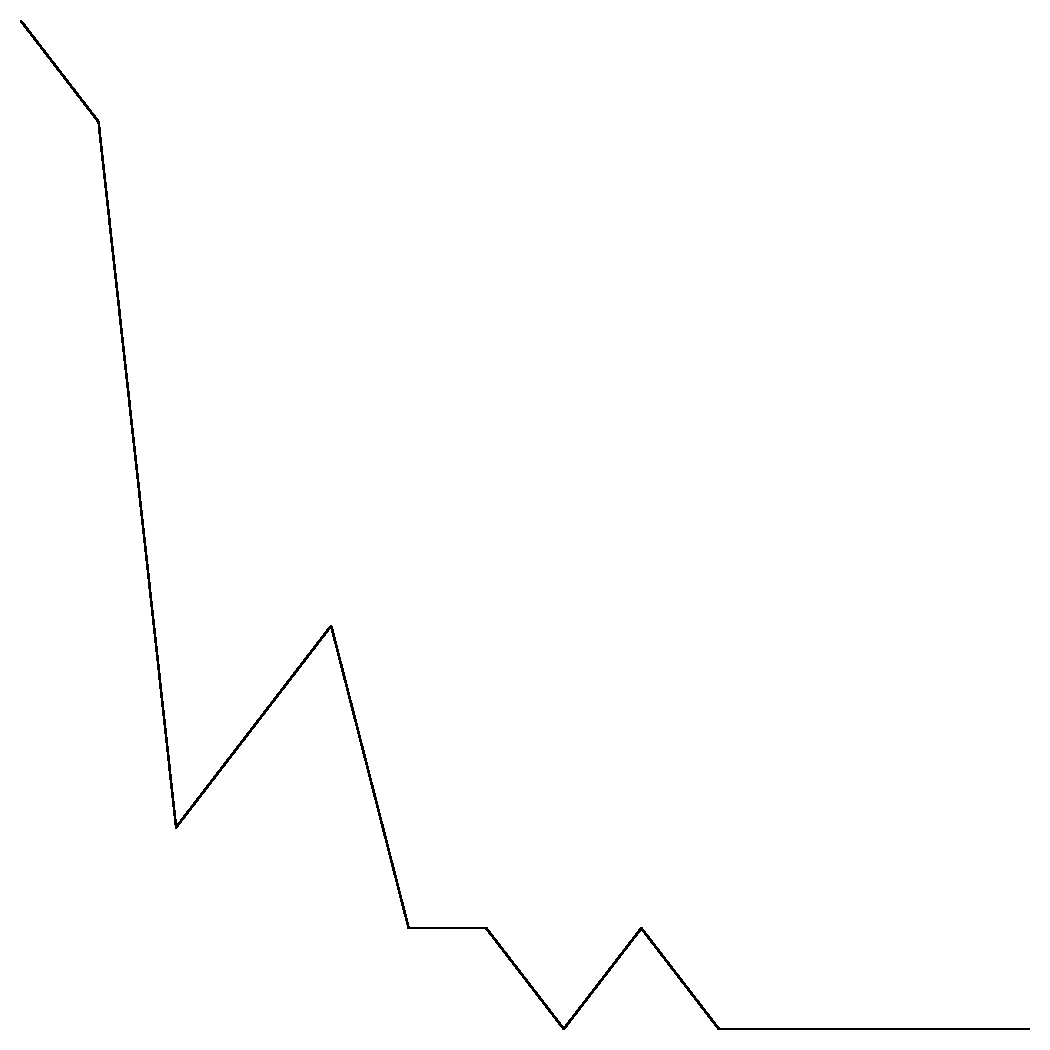
\includegraphics[height=10px, width=30px]{figures/sparkles/change-modified-API.pdf} & Changed API\\
&\vspace{-2pt}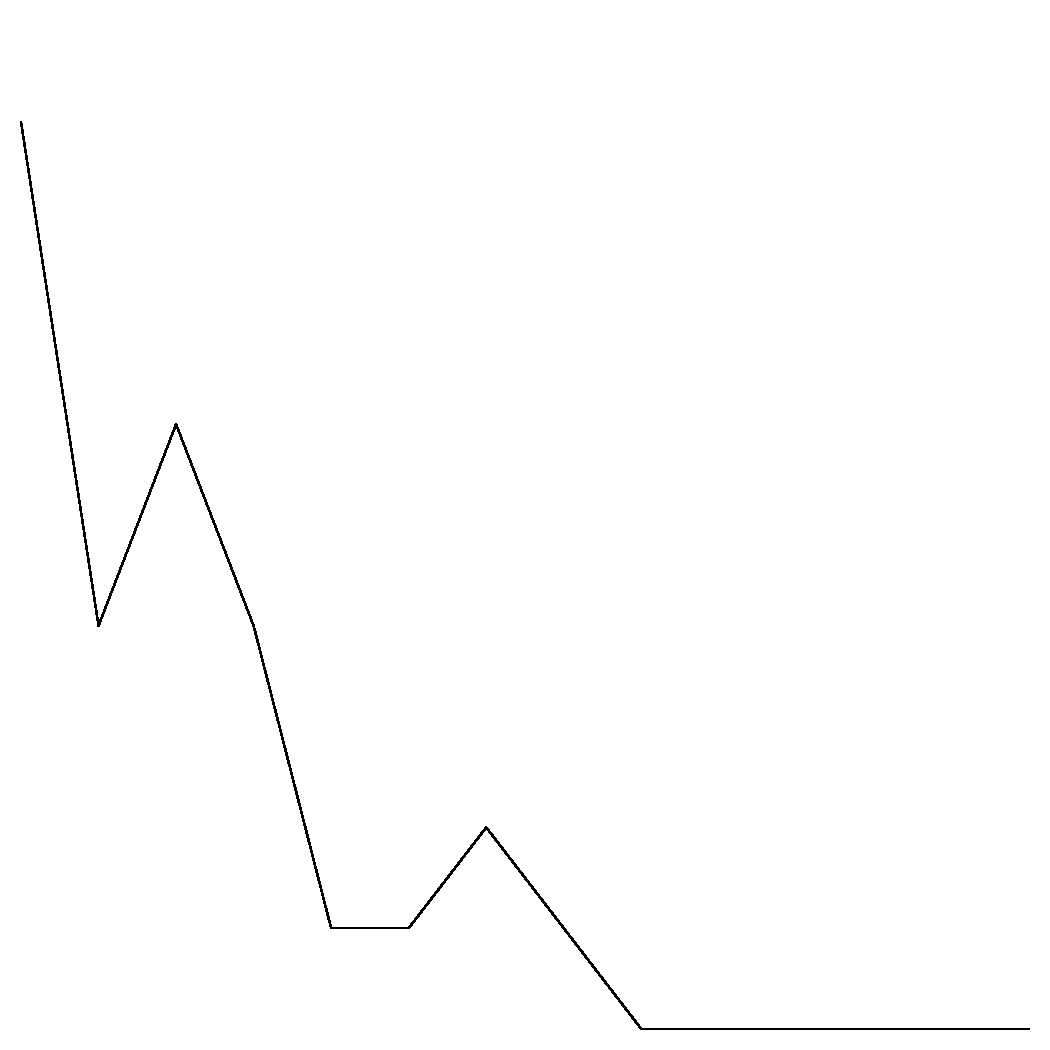
\includegraphics[height=10px, width=30px]{figures/sparkles/don-t-know-why-code-was-changed.pdf} & Don't know why code was changed\\
&\vspace{-2pt}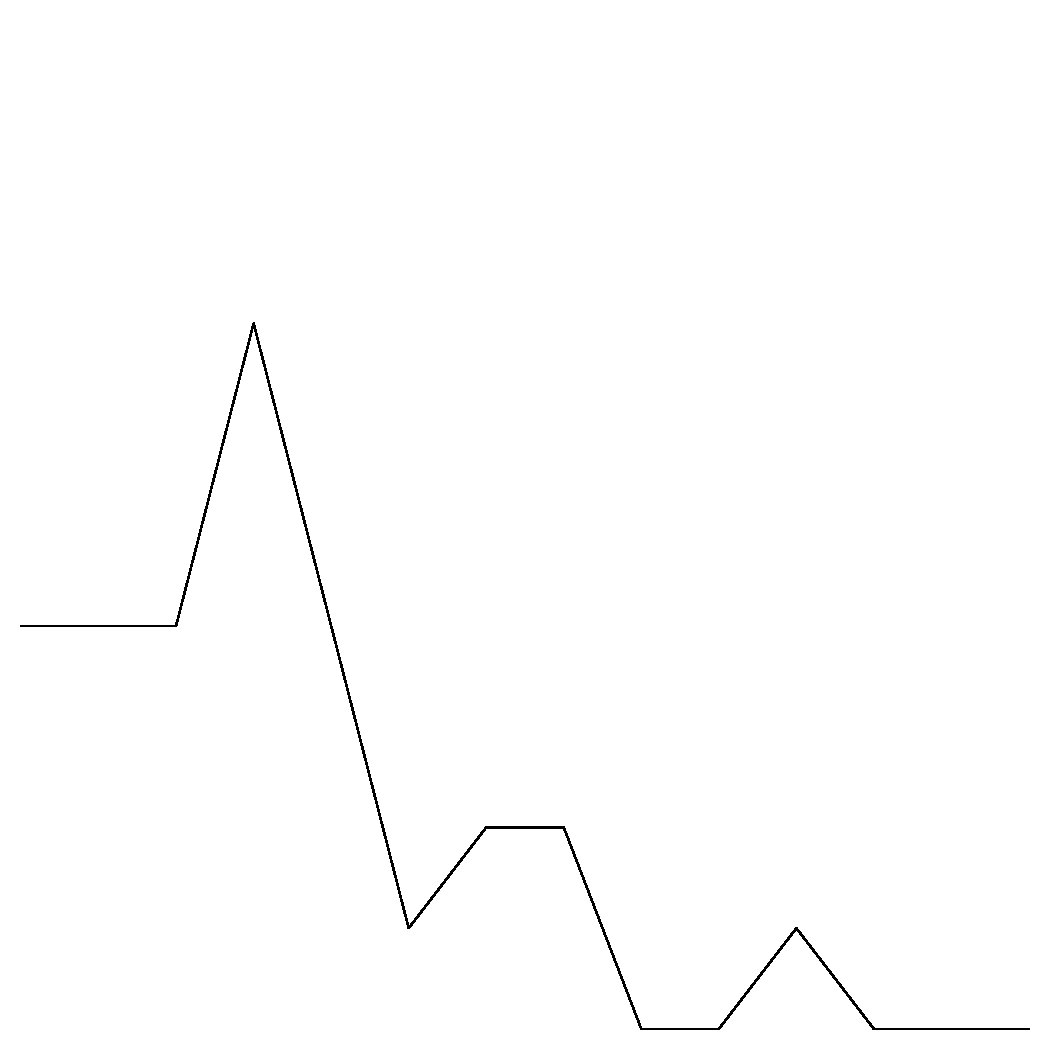
\includegraphics[height=10px, width=30px]{figures/sparkles/code-affects-frequently-used-features.pdf} & Affects frequently used features\\
&\vspace{-2pt}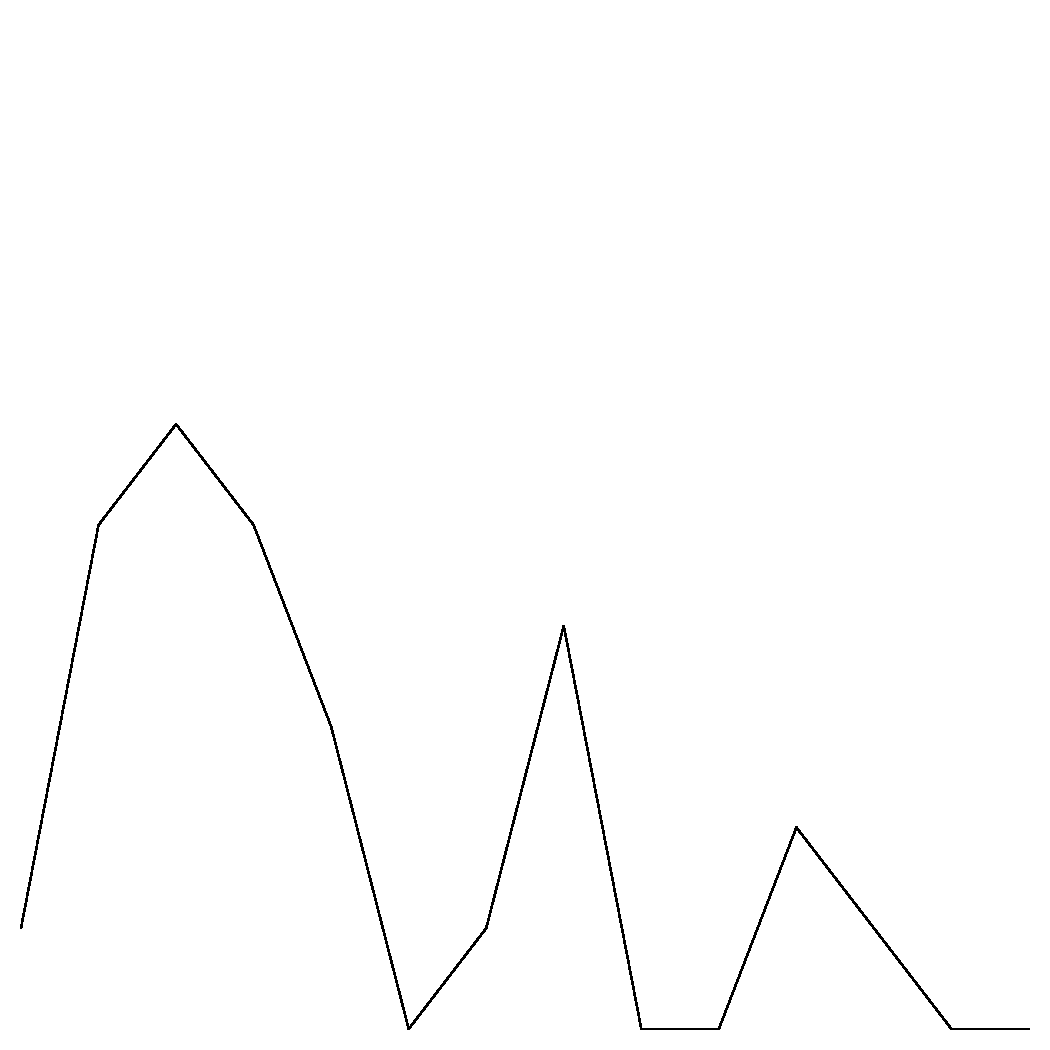
\includegraphics[height=10px, width=30px]{figures/sparkles/complex-code-was-changed.pdf} & Complex code\\
&\vspace{-2pt}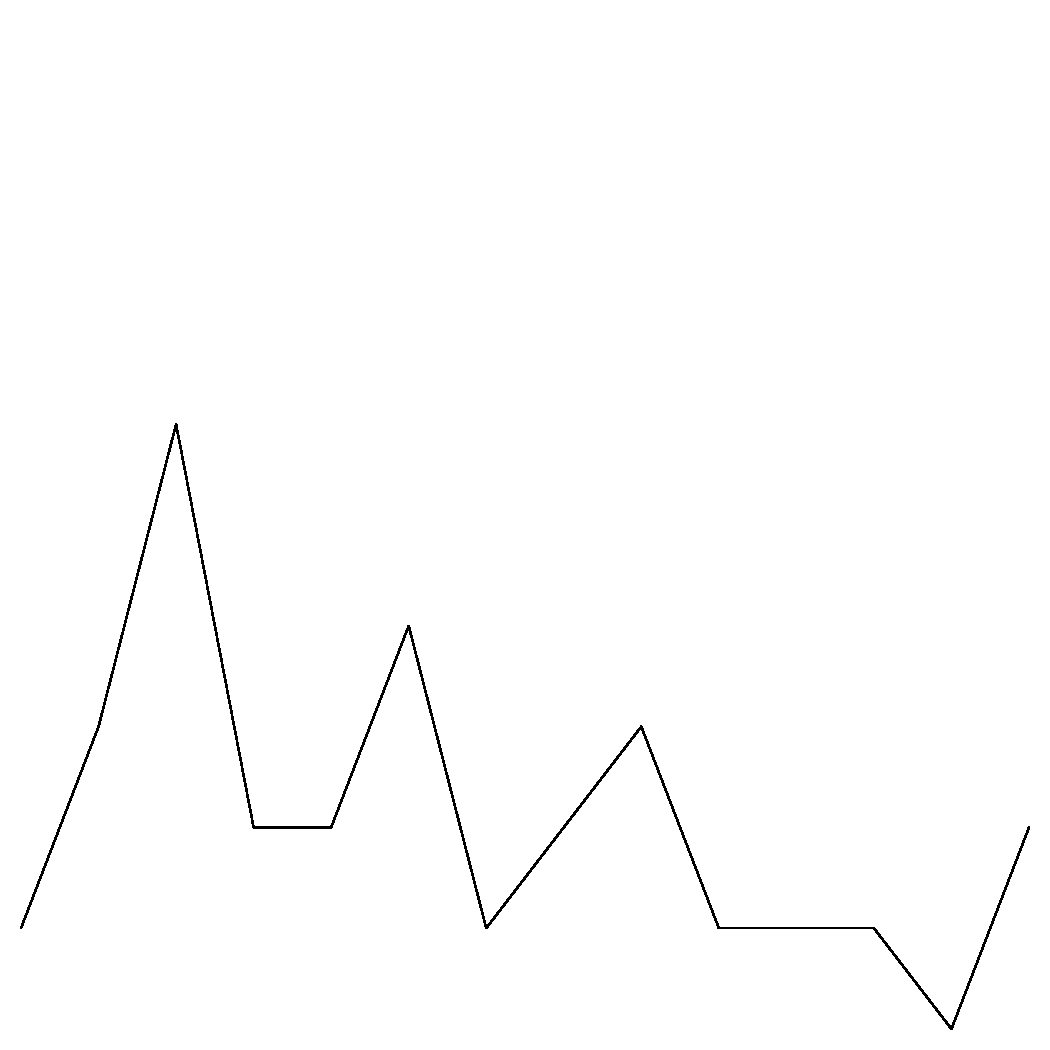
\includegraphics[height=10px, width=30px]{figures/sparkles/change-introduced-new-functionality.pdf} & Introduced new functionality\\
&\vspace{-2pt}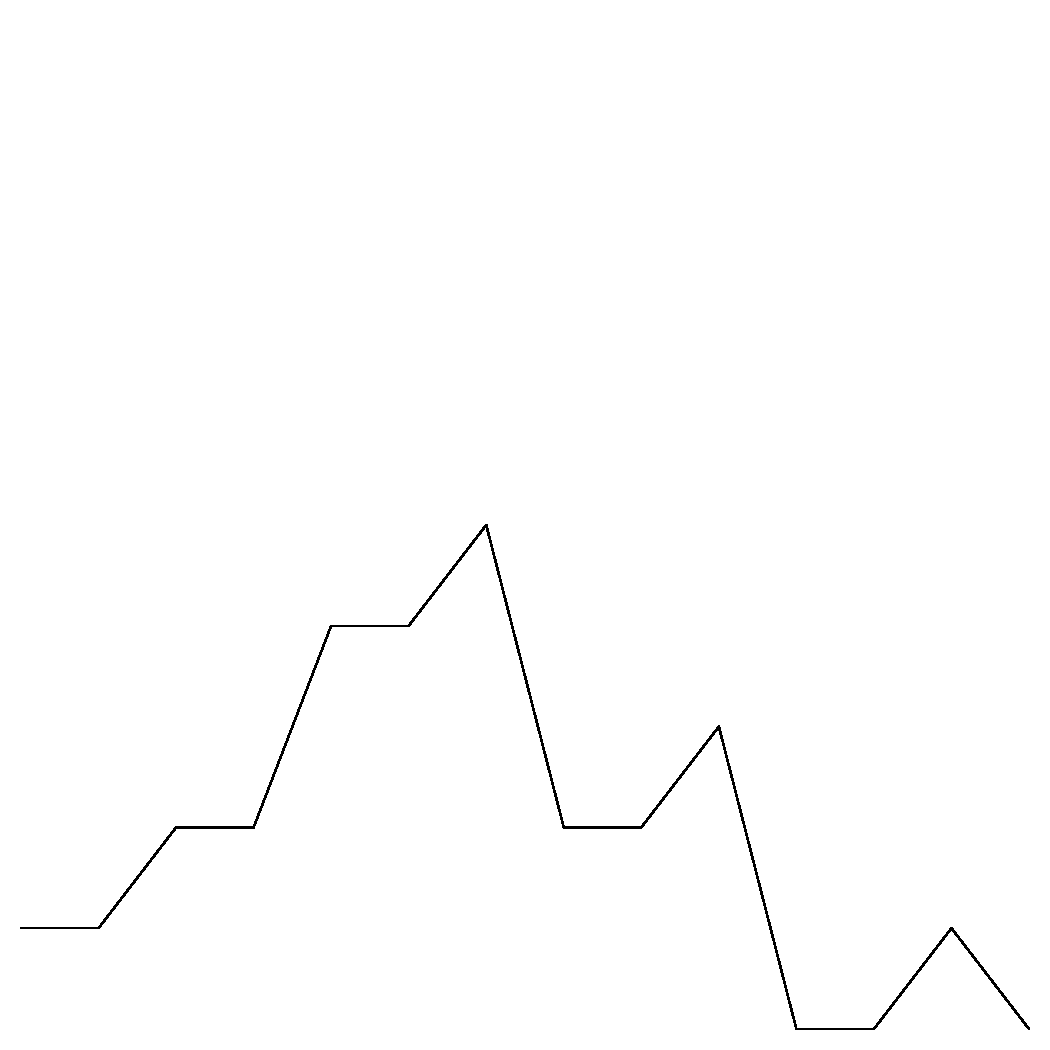
\includegraphics[height=10px, width=30px]{figures/sparkles/code-is-used-by-many-other-methods.pdf} & Is used by many other methods\\
&\vspace{-2pt}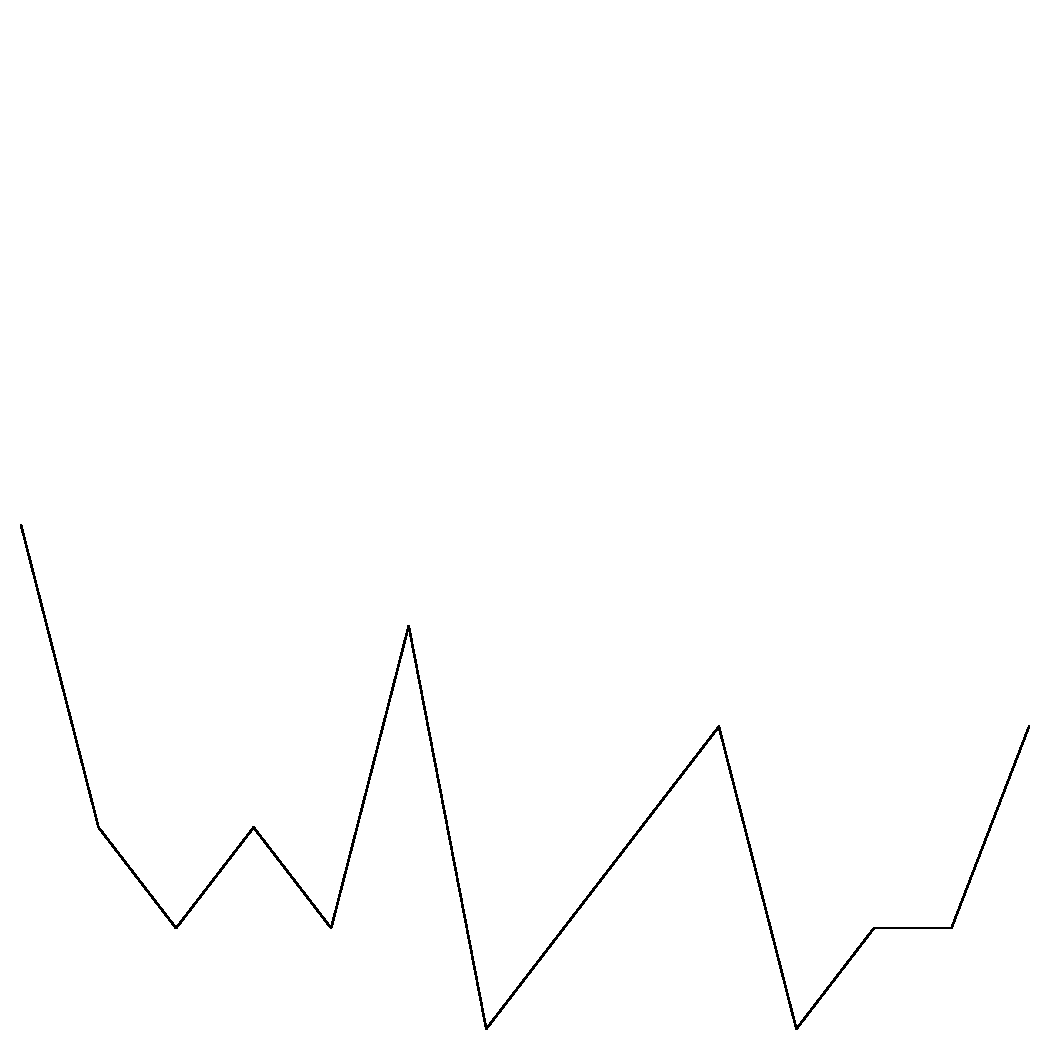
\includegraphics[height=10px, width=30px]{figures/sparkles/your-code-was-changed.pdf} & Your code was changed \\
&\vspace{-2pt}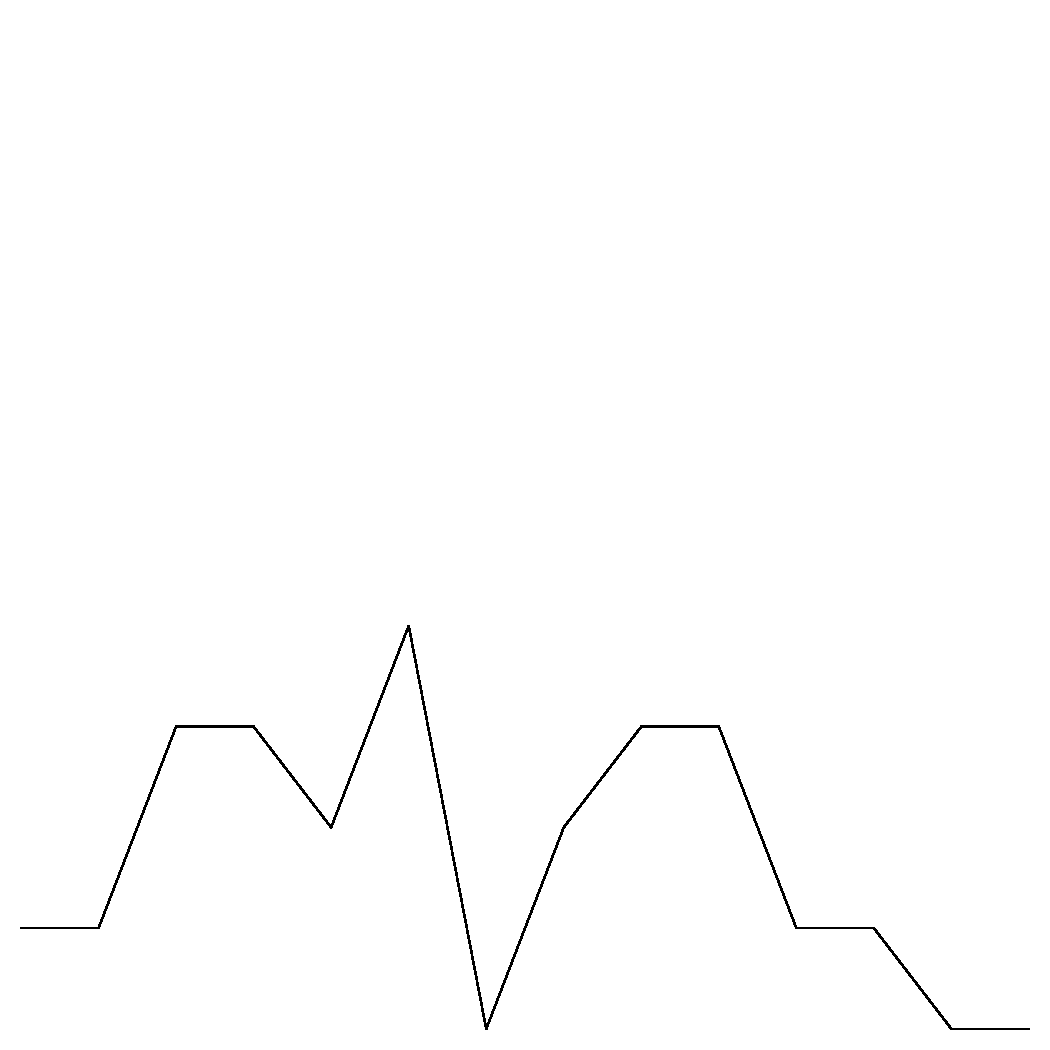
\includegraphics[height=10px, width=30px]{figures/sparkles/stable-code-was-changed.pdf} & Stable code was changed\\
&\vspace{-2pt}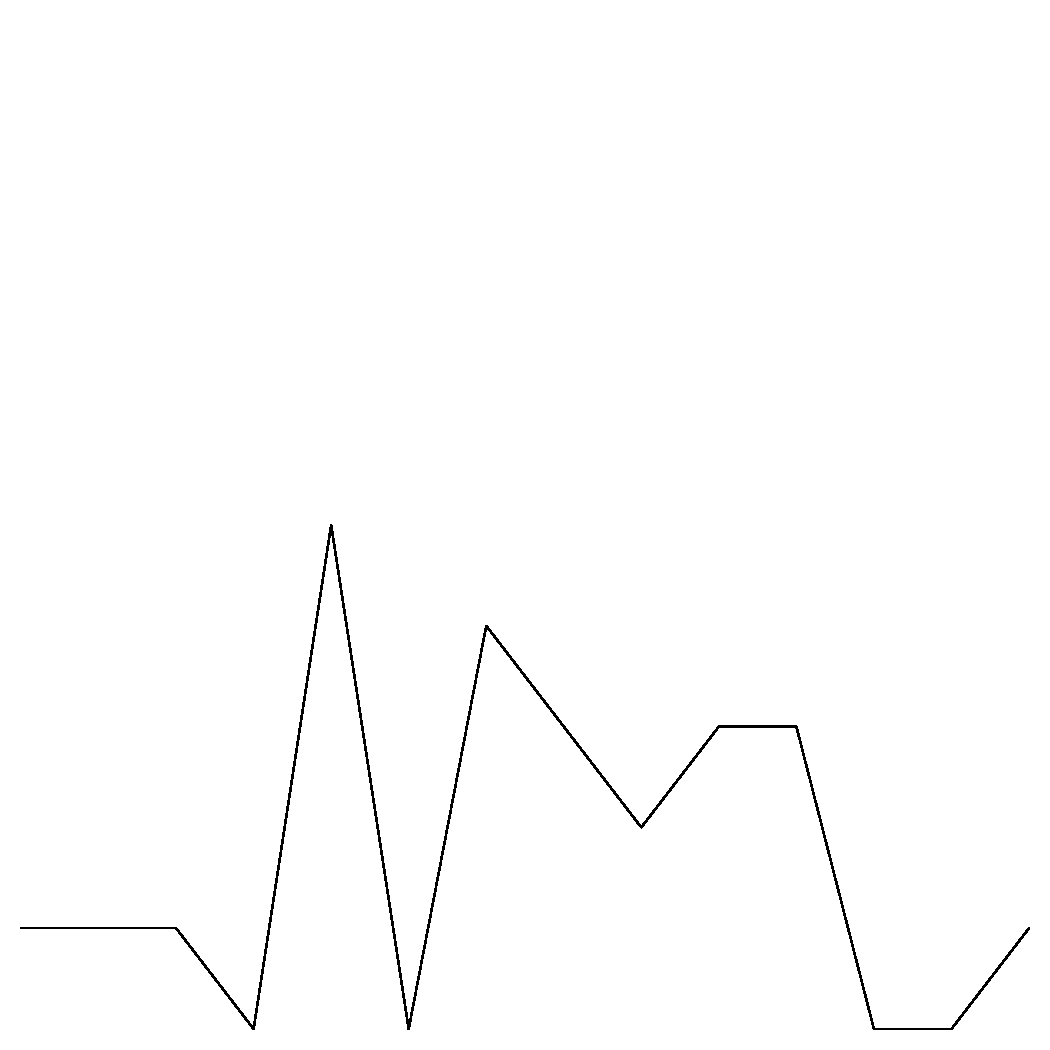
\includegraphics[height=10px, width=30px]{figures/sparkles/change-unlocks-previously-unused-code.pdf} & Change unlocks previously unused code\\\
&\vspace{-2pt}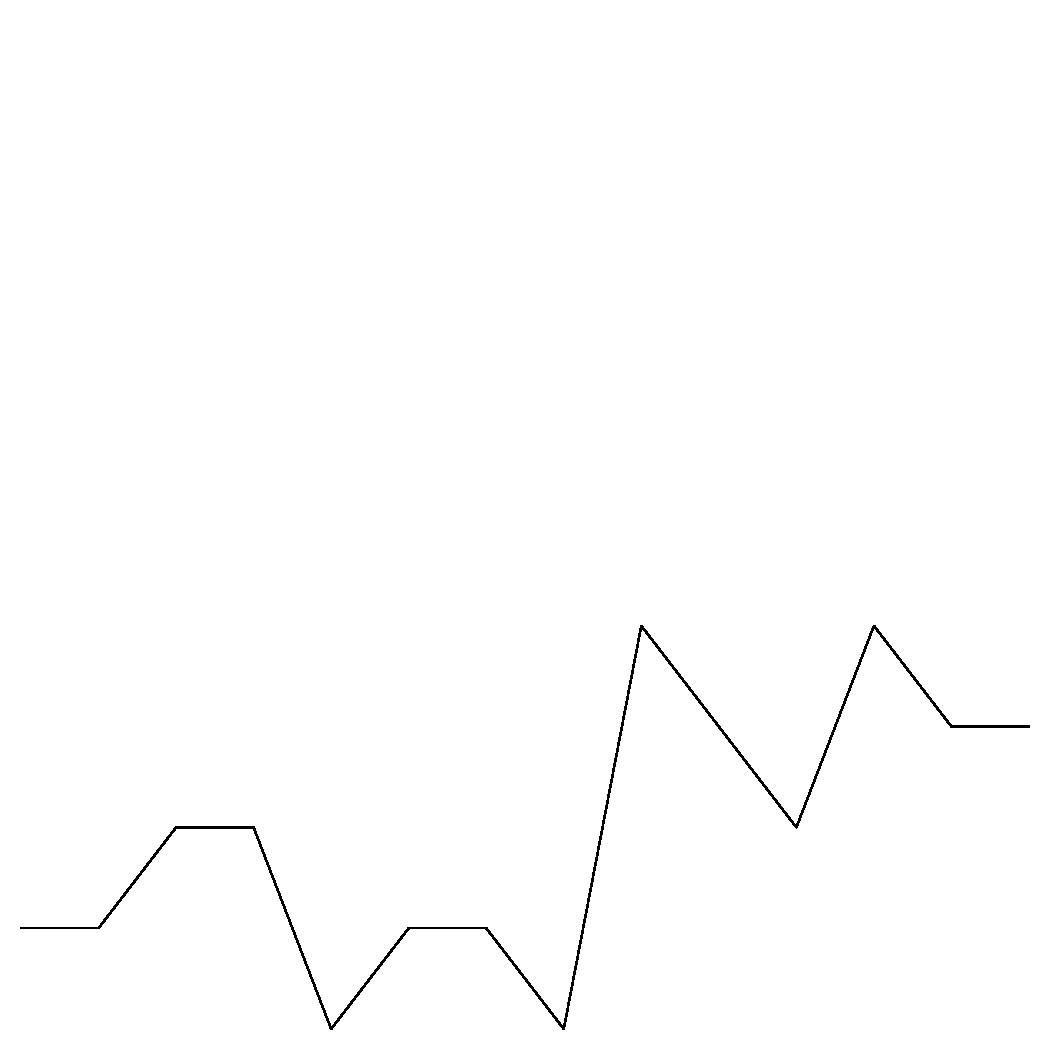
\includegraphics[height=10px, width=30px]{figures/sparkles/change-was-a-bug-fix.pdf} & A bug fix\\	
&\vspace{-2pt}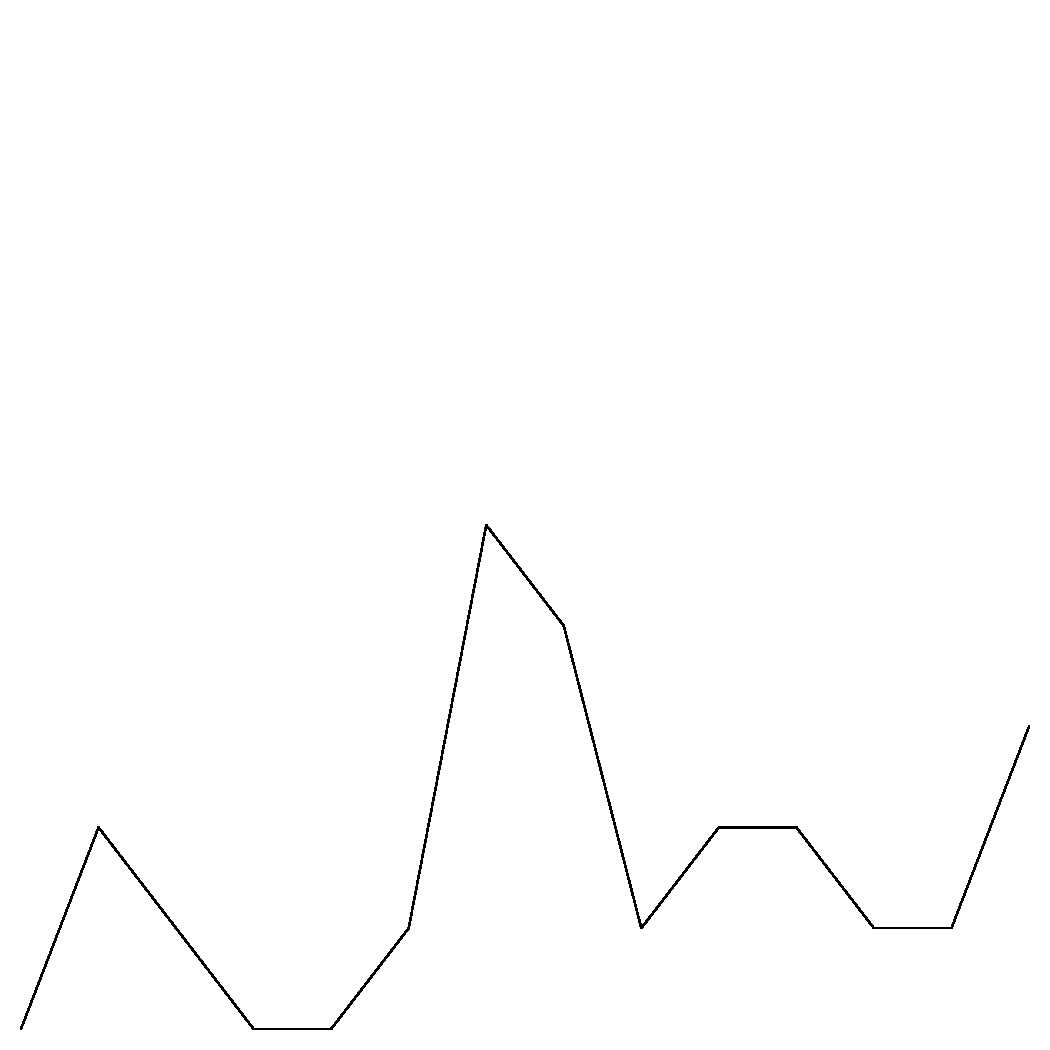
\includegraphics[height=10px, width=30px]{figures/sparkles/change-was-a-re-factoring.pdf} & A re-factoring\\ 
&\vspace{-2pt}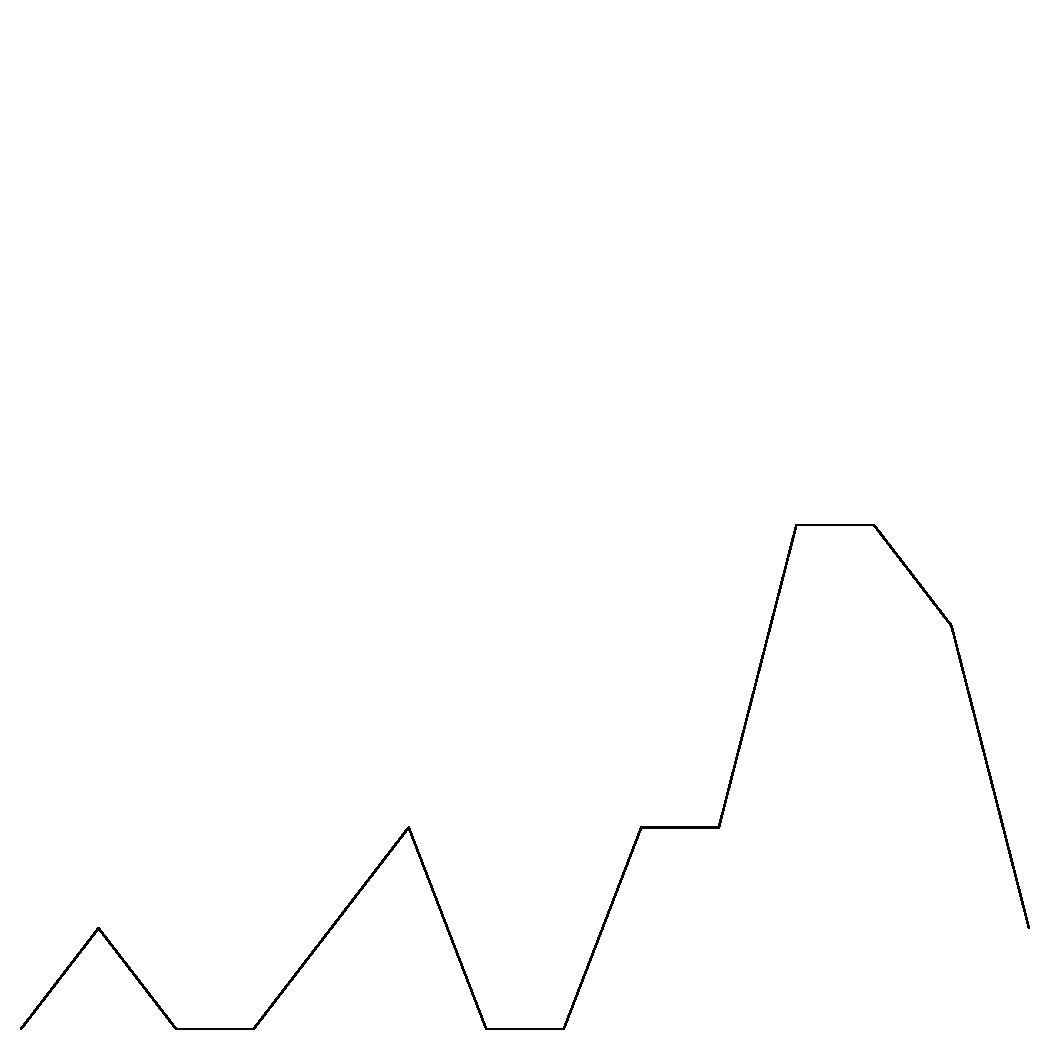
\includegraphics[height=10px, width=30px]{figures/sparkles/frequently-modified-code-was-changed.pdf} & Frequently modified code was changed \\
&\vspace{-2pt}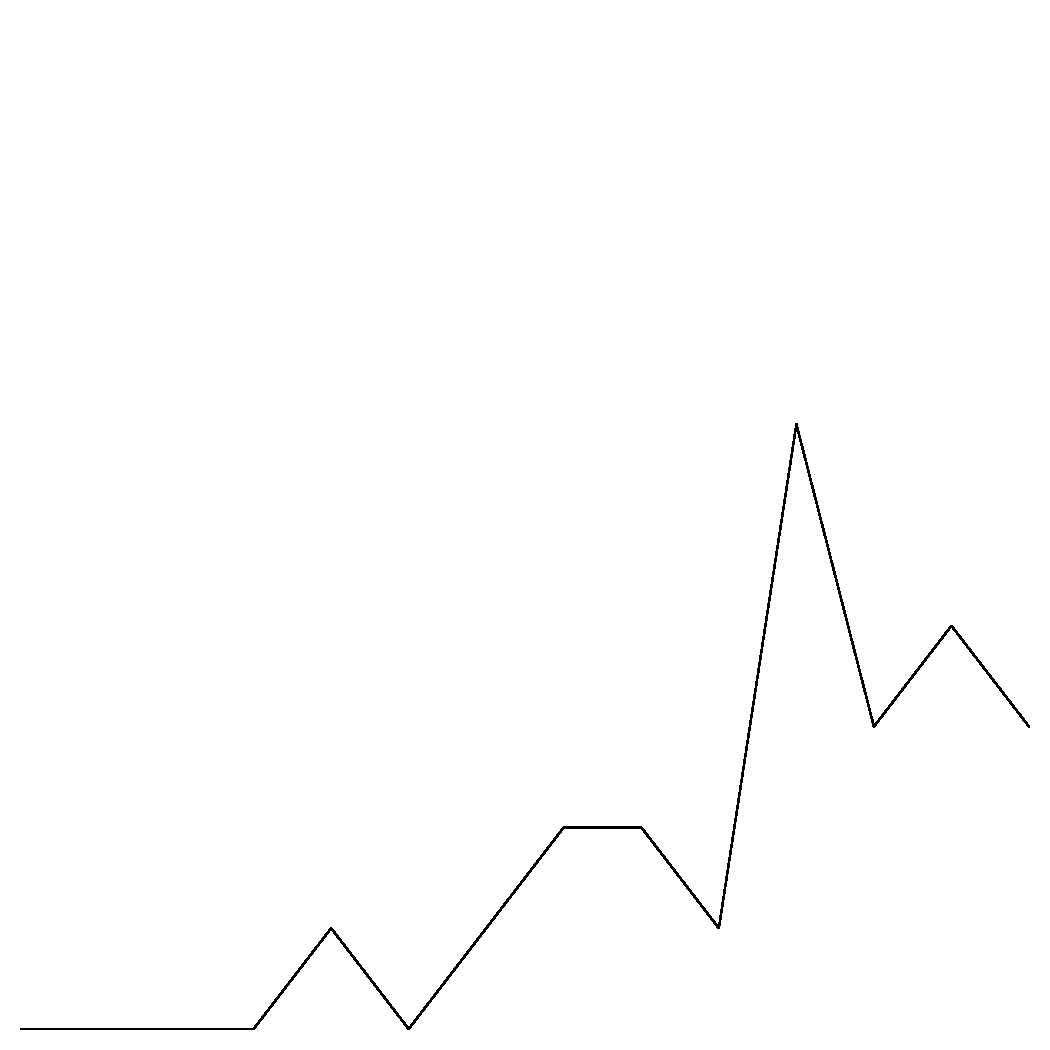
\includegraphics[height=10px, width=30px]{figures/sparkles/code-is-used-by-a-few-other-methods.pdf} & Code is used by few other methods\\ 
&\vspace{-2pt}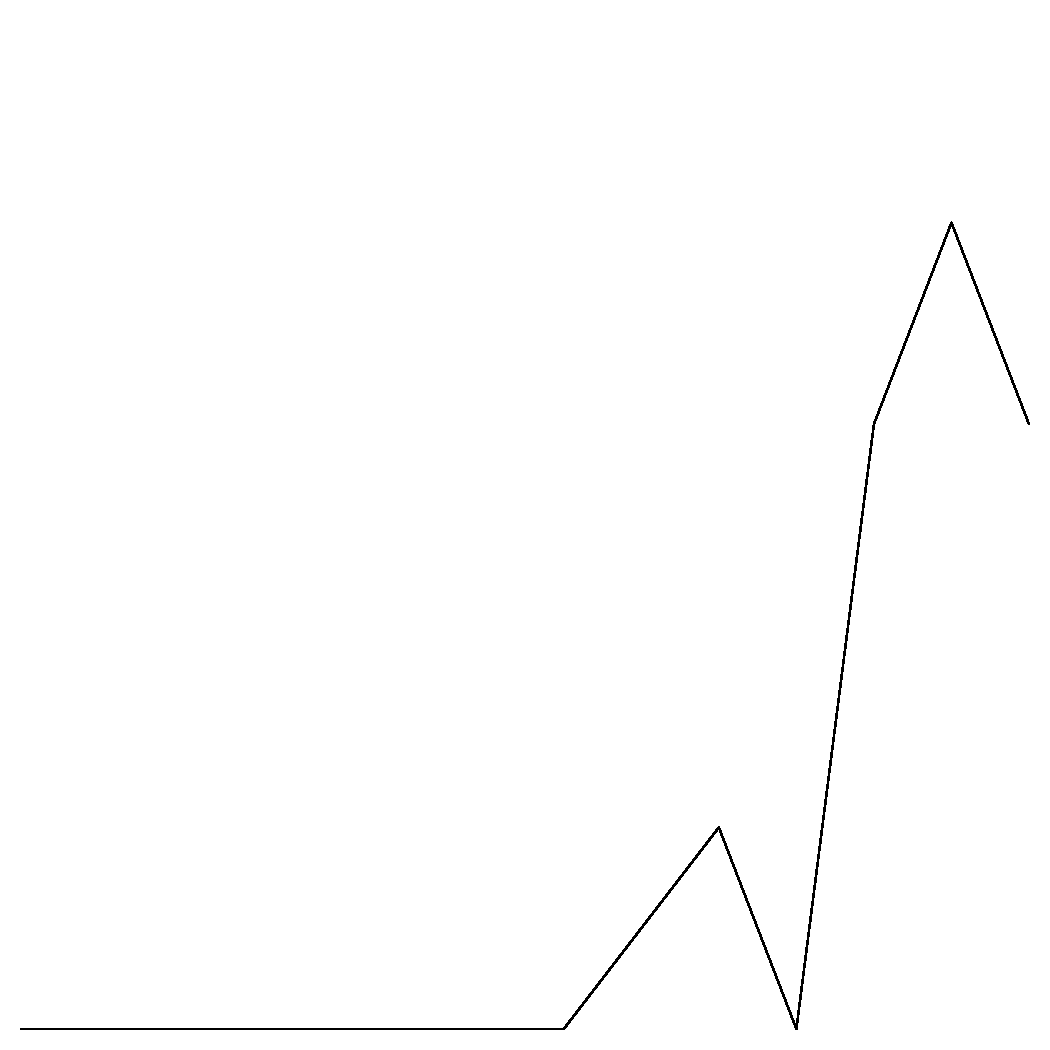
\includegraphics[height=10px, width=30px]{figures/sparkles/simple-code-was-changed.pdf} & Simple code was changed\\
\bottomrule
\end{tabular}
\vspace{-5pt}
\caption{This table contains the distribution of ranks for each survey item. The leftmost point of each sparkline represents the amount of respondents that ranked the item first; the rightmost point represents the amount that ranked it last (14th).}
\label{tab:sparkle}
\end{table}


\subsection{Development Mode}
One of the strongest findings from our study was the effect of the development mode that the team is in on its communication behaviour. Developers and managers alike give much importance to the development mode they are in, namely (1) normal iteration, and (2) endgame.

The normal iteration mode mainly consists of work that can be planned by the developer. This work tends to be new feature development, or modifications to existing features. Most of the planning for it has been laid out in advance; furthermore, each developer individually knows what features have been assigned to her, and can plan ahead to meet her obligations.
In contrast, the endgame mode mainly consists of work that is coming uncontrollably in short intervals from others. As a result of integration and more intense testing, defects crop up more rapidly and need to be addressed more quickly. Beyond allocating time for endgame activities, there is very little in this development mode that can be planned in advance.

The RTC team switches between the two modes in each iteration. Of the six weeks of a regular iteration, four weeks are assigned to normal iteration mode and two weeks to endgame. However, as deadlines approach, there are occasional special iterations that consist mostly of endgame-like work. In this manner, the same detailed pattern of alternation between normal iteration and endgame within an iteration is reproduced at a higher level, as shown in Figure~\ref{IterationsFig}.

We identified the same pattern with respect to the amount of changeset-related interactions in the team. We found that the mode in which the team is currently in is an important factor determining whether developers will feel a need to communicate about changesets. Being in endgame mode increases the need for developers to communicate about a changeset, whereas being in normal mode decreases the need to request information about it.

The first author of this paper experienced both modes during his participant-observer time with the RTC team. He joined the team in a release endgame phase, which was characterized by fixing bugs that were reported by testers, and he helped by fixing minor bugs as well as setting up servers for testing. When the team released the project, it switched gears, and in the decompression after the endgame he had the opportunity to develop a feature for the product. The differences in the patterns of interaction between the two modes were distinctly clear, for him and for his peers. During the endgame mode, developers were essentially ``on demand,'' available to fix whatever bugs were discovered. Later, during the normal iteration mode, they experienced far more autonomy and control over their time, and began working on activities that were less demanding of an interaction back-and-forth, and especially less demanding of keeping track of the changesets committed by their peers. In our interviews, developers almost unanimously pointed to the separation of the two types of modes, describing the differences in the type of communication in each, and identifying the autonomous \emph{vs.}~uncontrollable, inside \emph{vs.}~outside influence.

This is not to say that developers do not communicate while they are in normal iteration  mode, but that the nature of their communication seems to be different. In normal iteration mode, developers communicate less about concrete changesets, but they communicate more about high level ideas: for instance, they raise questions about how a feature fits into the existing architecture or general tactics to implement a feature, about how much of it actually needs to be implemented or can be reused from other libraries, and so forth. Generally, however, the amount of communication decreases in normal iteration mode. As a developer commented in one of our interviews, \emph{``during feature development iterations there are weeks I sometimes don't talk to my colleagues at all.''} 

In contrast, the endgame mode is characterized by bug reports and last minute feature requests---that is, by work coming into every developer's desk uncontrollably. Changesets become first class concerns during this mode because each change threatens the stability of the product: developers need to evaluate whether the changeset actually improves the product instead of making things worse. Therefore, they develop a habit of reviewing each other's changesets to assess the risk they pose to the project's stability.

Our survey data provides significant support for this finding. In Table~\ref{tab:sub-process}, we can see that overall, for the RTC development team at large, there is a greater likelihood to request information during product-stabilizing phases, such as 
\emph{during the release endgame}, and a lesser likelihood to request information when working towards an \emph{early milestone}. The former was ranked as the most important of the process-related items in our survey; the latter was ranked as the least important. All the survey items that refer to a late stage in the iteration or in the project lifecycle were ranked highly, and all the items that refer to an early stage were ranked lowly. This finding resonates especially with the team we interviewed. 


\subsection{Perceived Knowledge of the Changeset Author}
One key determinant for a developer to seek information about a changeset consists of what the developer knows about the background of its author. Several aspects of the author's background seem to be important: the quality of her recent work, her level of experience, and her awareness of recent team events or decisions.

First, these factors are important in part because they point to potential problems with the stability of the product. If a changeset author has \emph{recently delivered sub-standard work}, other developers will want to ensure that the new changeset will not deteriorate their product, and therefore they will try to find more information about it.

Similarly, when the author is \emph{inexperienced}, or is not \emph{up to date} with recent team events for any reason, the risk of introducing problems into the product increases. One developer that interacts frequently with a newly founded team told us that \emph{``most of the work that I need to review is of very low quality and needs several iterations before it is up to our standards.''} Novices, generally speaking, face a ramp-up problem that takes a significant amount of time to overcome~\cite{begel:sigcse:2008}. This was the case with Adrian's work, too: his first changesets were subjected to more scrutiny due to his unfamiliarity with the code base.

The survey data backs up these observations. The three top items in Table \ref{tab:sub-social} consist of factors related to an unfavourable perception of the background of the changeset author. In comparison, the two least important items in that table refer to favourable perceptions of said background.

In essence, these items point to the relevance of trust in software development teams. For developers, trust in the skills of their colleagues is important. If this trust is not-established (for instance, if a developer does not know the changeset author), developers are more likely to check the changeset and request information to ensure that the modifications were truly necessary and appropriate. But when trust exists (that is, when the author has a good record of delivering high-quality work, or is known to be an experienced team member), the need to seek information about a changeset decreases. 


\subsection{Common Experience and Location}
Shared work experiences affect the likelihood of information-seeking behaviour in the RTC distributed team. This is partly related to the trust and perception issues discussed above, but also to the establishment of interpersonal relations and to the intertwining work responsibilities and expectations.

According to our interviews, this is the case particularly for senior team members. Although they work in a globally distributed team, they have managed to establish personal relationships with developers at many different sites. Through continuous interaction and through social events, they have learned more about each other, and thus feel more comfortable to initiate contact with them. Junior team members, in contrast, know very few of their teammates globally, and since they simply do not have these interpersonal connections with the rest of their team, it is less important to them whether they know the author of a changeset when needing to contact them.

Generally speaking, despite the lack of opportunities to build personal relationships with off-site people, for most developers sharing common experiences makes it easier to contact teammates to request information. One team lead told us: \emph{``I have one or two contact people in each team we usually work with whom I ask for information and then often enough get referred to the right person in their team.''}

Our participant-observation data confirm this. At one point, Adrian needed to set up and test a specific component in the RTC product. The development team in charge of that component was located on a different site. However, since Adrian had previously had the opportunity to establish relationships with some of the developers of that team through a previous research study, it was easier for him to contact them and ask for help in his setup task.

Our survey data corroborate these observations. It suggests that the developers that form relationships (on a personal or work level) with other developers gave more emphasis on previous experiences with them. For instance, it made a difference whether the developers \emph{are currently working together} (Table~\ref{tab:sub-social}). Additionally, whether they have shared work experiences seems to be a more determinant factor than having \emph{met in person} or sharing the same \emph{physical location}.

This last finding would seem to indicate that the RTC team has managed to overcome obstacles created by geographical distance. Developers state that the physical location of a changeset author is not an important factor to seek more information about the changeset. Nevertheless, we should note two things. First, this finding merely points out that developers have no greater need to inform themselves of work output of their remote peers than of their local peers; it says nothing about the ease with which such information is acquired. Second, the RTC team has determined to carry out as many of its interactions as possible through textual, electronic media. This neglects the natural advantages provided by proximity in favour of uniform accessibility of interactions, no matter the physical location of the interlocutors.



\subsection{Risk Assessment}
A central factor at the heart of the decision to seek information is a concern with the quality of the product and components developed by the team at large. Both managers and developers share this concern. Because of it, every team member is constantly evaluating whether there are significant risks involved in accepting a changeset and including it into the final product. This concern is greatest close to releases or major milestones, and less important when the team is in normal iteration mode.

Developers request information more frequently about changesets that touch on code that has a high customer impact. According to our interviews and observations, code parts with a high customer impact are those that are directly related to frequently used features or changes to the API that might be used by customers to customize the RTC product. In the case of the impact of API changes, there is an extensive knowledge exchange in the jazz.net forums between customers and developers about how to use the API to build extensions to RTC, which gives developers plenty of information about the possible impact of API changes to the customers. Consequently, changesets that modify code that has less impact on the customer are of less concern and less likely to be discussed. For example, when scanning fixes to reported bugs, developers perform a risk assessment to determine whether the bug fix is even needed. In the words of one team member, \emph{``with every tenth bug fix you introduce another bug to the system, so unless the bug does not have a workaround and is something most customers would experience, we give it low priority.''}

The ranking of items in Table \ref{tab:sub-technical} provides additional insights into the kinds of changesets that carry a risk for developers. A \emph{changed API} comes at the top of the list, code that \emph{affects frequently used features} comes third, immediately followed by changes to \emph{complex code}, changes that \emph{introduced new functionality}, and changes to code that \emph{is used by many other methods}.


\subsection{Work Allocation and Peer Reviews}
In the later stages of the development cycle, developers have two process-based constraints that prompt them to interact with their peers. First, they need their peers to review their changesets before they are included in the product. Second, they need an approval to start working on a task (a triaging process needs to take place so that developers are allocated to the most important work items).

In the changeset review process, there are two ways the changeset author and the reviewers interact.
Either the changeset author submits his changeset for review, or the changeset author discusses the changeset with the reviewer before submitting it for review. The main discriminant between meeting with the reviewer to discuss the changeset before submitting it or submitting without prior discussion seems to be whether the reviewer and the author are co-located.

Adrian's mentor during his time with the RTC team explained: \emph{``It is very demotivating to get a changeset rejected, that's why we usually try to discuss things before and then the reviewing just becomes all about quickly testing and accepting the changeset.''} Of course, this does not prevent an already discussed changeset from being rejected, but it signals that the process-based constraint is not as strict as to forbid discussions about a changeset between authors and reviewers in the interest of an unbiased code review.

In the case of developers seeking approval to start working on a task, the process is similarly flexible. The approval is supposed to be issued before the developer begins work on the task. However, we observed several times that developers performed quick fixes, and later went to their team leads to acquire approval for the fixes they had already performed.

Several items in our survey point to the importance of information-seeking around the processes of approval and peer review. In Table \ref{tab:sub-process}, the second- and third-highest items were information needed because the respondent needed \emph{to review the change} or \emph{to approve the change}. The need to  \emph{obtain a review for the change} or to \emph{obtain an approval for the change} were of moderate importance. \emph{Verifying a fix} was not judged as important by our respondents.

\subsection{Type of Change}
The three main reasons for a developer to commit a changeset are to (1) do feature development, (2) fix bugs, and (3) re-factor. Among them, feature development seems to be the one that prompts developers to seek information the most.
In our survey (Table \ref{tab:sub-process}), code that \emph{introduced new functionality} is ranked fifth among the code-change related factors, while changes that consist of \emph{a bug fix} and \emph{a refactoring} ranked far lower on the same list.

This may be due to the fact that feature development has less tool support than bug fixing (which is supported by debugging tools and automated test frameworks) and refactoring (which is essentially an automatic process today). The limited tool support and the inherently difficult nature of the task itself makes changesets that introduce new functionality more difficult to understand or assess. Hence, developers are more likely to request information about them.


\subsection{Business Goals vs Developers' Pride}
Senior team members (managers and team leads among them) often ask about the purpose and the real need of a changeset in order to minimize unpleasant surprises that might be introduced with further code changes, and simply to have an economically feasible product. One senior development lead told us: \emph{``often I need to stop my developers from fixing every little bug otherwise we would never be able to ship.''}

Although every team member is concerned with the quality of their product, a more realistic, business-oriented perspective seems to be more prominent in the senior team members' information-seeking behaviour: they may request clarifications on the business case of changesets or work items if they are not immediately clear in the existing documentation.

More junior team members, however, do not have this concern. They express their pride in the actual product and want it to be as bug free as possible. A developer commented to us: \emph{``I want to be proud of what I deliver and I am fairly certain if we don't fix it now it will come back to haunt us because it might upset some customers.''} Not only does this lead the developer to try to convince her manager that including changesets for seemingly unimportant fixes is valuable, it also makes her information-seeking behaviour different with respect to that of the more senior team members. Broadly speaking, managers will be more interested in seeking clarifications as to the business case of a work item if it is not clear in its description, while developers will not care as much about this.

\section{Recommender System Design Guidelines}
\label{sec:sub:tools}
Nakakoji \emph{et al.}~\cite{nakakoji2010:rdc} formulated nine design guidelines for systems supporting information-seeking in software teams. Some of them deal with minimizing the interruptions experienced by the developers who are asked for information, while others refer to enabling the information-seeker to contact the right people. Our findings help us refine Nakakoji \emph{et al.} guidelines:


\textbf{Guideline \#1}: \emph{Recommender systems should adjust to the development mode.}
Our first finding strongly suggests that a developer's information needs can dramatically change between development modes. 
%
When in normal iteration mode, developers act upon planned work and can therefore anticipate the information they need, but in endgame mode, developers react to unplanned incoming work, such as bug reports or requests for code reviews. 

Many tools, such as Codebook~\cite{begel:icse:2010} and Ensemble~\cite{xiang:rsse:2008} provide information and recommendations in a fixed way. 
Codebook enables developers to discover other developers whose code is related.
In contrast,  Ensemble provides a constant stream of potentially relevant events for each developer.
In the Codebook case, this might lead to extra overhead in endgame mode when developers frequently need to search for information instead being automatically provided, whereas Ensemble might overload developers during the feature development mode by providing a constant stream of information.

To avoid overwhelming or reducing overhead further for developers, recommendation systems should either automatically adjust to the development mode or feature customizable templates that can easily be switched. 

\textbf{Guideline \#2}: \emph{Recommender systems should account for perceived knowledge of other developers.}
Our second and third findings unveiled factors that trigger developers to seek information about a changeset that are not related to its code. 
Instead, developers pay close attention to the experience level as well as the quality of previously delivered work to determine whether to talk to the changeset owner.

Traditional recommender systems in software engineering focus on the source code to determine useful recommendations, e.g. Codebook~\cite{begel:icse:2010} and Ensemble~\cite{xiang:rsse:2008}.
This might lead to providing developers with information about changes that are of little interest due to the trust placed in more experienced developer. 

But because developers often look beyond source code and perform an additional step, namely considering the changeset owner's experience and recent work, information solely created from source code might miss interesting instances where novices to the code made inappropriate changes.
Recommender systems might report issues that are of less importance due to the substantial experience of the changeset owner.

Implementing filtering mechanisms based on author characteristics such as experience and quality of previously delivered work can help developers focus on the information that is important to them.


\textbf{Guideline \#3}: \emph{Recommender systems should assist in non-implementation tasks such as code reviews and risk assessment.} 
We observed, as described in the fourth, fifth, and sixth findings, that developers are highly engaged in discussions when performing risk assessments or reviews of changesets. 

In software engineering, most recommendations are focused on providing information to support concrete tasks such as bug fixes or re-factorings, but not for tasks such as reviews. To provide information for non coding tasks, recommender systems should be configurable to display relevant information beyond the tasks that they are intended to support, so that developer can easily access the information provided by recommender systems when performing code reviews or risk assessments.

\textbf{Guideline \#4}: \emph{Recommender systems should account for business goals.}
Our last finding points to internal conflicts within teams and among developers caused by the desire to create a flawless product under the restriction of a set of business goals such as shipping the product on time.
Thus, developers often need to be reminded that they must focus their efforts on fulfilling business goals rather than on polishing the product as they see fit. Existing recommenders that use code-related metrics such as quality or productivity may shift attention away from fulfilling business goals.

To support developers in focusing on business goals, systems supporting the information-seeking behaviour of developers should be able to prioritize information related to tasks that are mission-critical to the organization, helping the team focus its attention on the most relevant problems for the upcoming release.

\section{Threats to Validity}
\label{sec:threats}
Our survey asked the developers to rank a pre-defined list of items in
terms of the influence they may have on their information-seeking behaviour.
In doing so, we attempted to reach a compromise between the survey length and
survey response rate. 
This bias poses a threat to our findings due to the possibility that we were missing important items.
We mitigated it by developing the survey iteratively by piloting and discussing it with one of the development teams to identify the most important items, and by relying on our other two sources of data to triangulate our findings.

We had the chance to interview ten developers, which represent a fraction of the development team at large. These ten developers were all located at the same site. As a result of this, our interview data could be biased and unrepresentative of the RTC team at large.
However, we are confident that this threat is minor, due to the mix of developers we interviewed, including novices, senior developers, and team members that had been part of the group since its beginning.
Furthermore, triangulation with our observations and survey responses increases our confidence in our findings.
However, we plan to interview team members from other locations to minimize the cultural (national and local corporate culture) bias that might have been introduced by focusing the interviews on one location. 

Our data come exclusively from the IBM RTC development team, and the extent to which our results are valid for other companies is not clear without replications. 
The RTC development team has more than one hundred members, it interacts with a number of customers, and it is in the process of integrating its product with others.
These are all forces that shape communication dynamics. 
However, their interaction patterns seem to be similar to those of other globally distributed teams that need to synchronize work across multiple time zones.

\section{Conclusion and Future Work}
\label{sec:conclusions}
We end this chapter by bringing it back to the initial research questions we set out to answer:
\begin{description}
  \item[RQ 2.2:] Do developer accept recommendations based on software changes to increase build success? 
\end{description}

The findings we presented in Section~\ref{sec:findings} show that there are different factors that influence developer to investigate about change-sets.
Although not directly asked for, the developer with reporting on those factors answered our research question in a positive way.
We found that developer do talk about change-sets which represent our level of recommendations as well as they show interest in build outcome towards the end of a release cycle.
Thus the developer answers both validated that they would accept recommendations both in the form we present them, namely per change-set submitted, as well as lending our outcome metric more credibility as they show a keen interest in build success when the date to ship the product approaches.

In the next chapter we return to our path of a more direct analysis of our recommendations by showing a proof of concept that the recommendations do not only statistically relate to build outcome but that recommendation could actually prevent build failures.